\documentclass{beamer}
%
% Choose how your presentation looks.
%
\usepackage[T1]{fontenc}
\usepackage[utf8]{inputenc}
\usepackage{lmodern}  
\usepackage{amsmath}
\usepackage{bm}
\usepackage{booktabs}
\usepackage{multirow}
\usepackage{graphicx}
%
% For more themes, color themes and font themes, see:
% http://deic.uab.es/~iblanes/beamer_gallery/index_by_theme.html
%
\mode<presentation>
{
  \usetheme{Darmstadt}      % or try Darmstadt, Madrid, Warsaw, ...
  \usecolortheme{default} % or try albatross, beaver, crane, ...
  \usefonttheme{serif}  % or try default, serif, structurebold, ...
  \setbeamertemplate{navigation symbols}{}
  \setbeamertemplate{caption}[numbered]
  \setbeamertemplate{headline}{}
}
%
%
\title[Block 1]{Block 1 \\  Repetition from BSc courses  \\ LRM estimators \& non-linear extensions\\ Predictions from regression models}
\author{Advanced Econometrics 4EK608}
\institute{Vysoká škola ekonomická v Praze}
\date{}

\begin{document}
 
\begin{frame}
  \titlepage
\end{frame}

% Uncomment these lines for an automatically generated outline.
\begin{frame}{Outline}
  \tableofcontents
\end{frame}

%------------------------------------------------------
\section{Estimation methods, predictions from a model}
\subsection{Ordinary least squares}
\begin{frame}{Linear regression model (LRM) and OLS estimation}
$$
\bm{y} = \bm{X\beta} + \bm{\varepsilon}
$$
\textbf{LRM assumptions (for OLS estimation):}\\
(Notation follows Greene, Econometric analysis, $7^{\textnormal{th}}$ ed.)
\medskip
\begin{enumerate}
    \item[A1] \textbf{Linearity:} $y_i = \beta_1 + \beta_2 x_{i2} + \dots + \beta_K x_{iK} + \varepsilon_i$ \\LRM describes linear relationship between $y_i$ and $\bm{x}_i$.
    \item[A2] \textbf{Full rank:} Matrix $\bm{X}$ is an $n \! \times \! K$ matrix with rank $K$.\\ Columns of $\bm{X}$ are linearly independent and $n \geq K$.
    \item[A3] \textbf{Exogeneity of regressors:} $E[\varepsilon_i | \bm{X}]=0$ (strict form). \\If relaxed to contemporaneous form in TS: $E[\varepsilon_t | \bm{x}_t]=0$.\\Law of iterated expectations: $E[\varepsilon_i | \bm{X}]=0 ~\Rightarrow~ E[\varepsilon]=0$.
    %\\Also, we assume disturbances convey no information on each other: $E[\varepsilon_i|\varepsilon_1,\dots,\varepsilon_{i-1},\varepsilon_{i+1},\dots,\varepsilon_n]=0$.
\end{enumerate}
\end{frame}
%------------------------------------------------------    
\begin{frame}{Linear regression model (LRM) and OLS estimation}
$$
\bm{y} = \bm{X\beta} + \bm{\varepsilon}
$$
\textbf{LRM assumptions (continued):}
\medskip
\begin{enumerate}
    \item[A4] \textbf{Homoscedastic \& nonautocorrelated disturbances:}$$E[\bm{\varepsilon\varepsilon}^{\prime}]=\sigma^2\bm{I}_n$$ Homoscedasticity: $\textnormal{var}[\varepsilon_i|\bm{X}]=\sigma^2, \qquad \forall~i=1,\dots,n$.\\Independent disturbances: $\textnormal{cov}[\varepsilon_t,\varepsilon_s|\bm{X}]=0, \qquad \forall~t \neq s$.\\ \smallskip 
    \tiny{
    \begin{itemize}
        \item GARCH models [i.e. ARCH(1): $\textnormal{var}[\varepsilon_t|\varepsilon_{t-1}]=\sigma^2+\alpha \varepsilon_{t-1}$] do not violate the conditional variance assumption $\textnormal{var}[\varepsilon_i|\bm{X}]=\sigma^2$. However, $\textnormal{var}[\varepsilon_t|\varepsilon_{t-1}] \neq \textnormal{var}[\varepsilon_t]$, with conditioning on $\bm{X}$ omitted from notation but left as implicit.
    \end{itemize}}
    \normalsize
    \item[A5] \textbf{DGP of \textit{X}:} Variables in $\bm{X}$ may be fixed or random.
    \item[A6] \textbf{Normal distribution of disturbances:} $$\bm{\varepsilon} | \bm{X} \sim N[\bm{0}, \sigma^2\bm{I}_n].$$
\end{enumerate}
\end{frame}
%------------------------------------------------------
\begin{frame}{Ordinary least squares (OLS)}
\vspace{-0.3cm}
$$
\bm{y} = \bm{X\beta} + \bm{\varepsilon}
$$
\medskip
The least squares estimator is unbiased (given A1 -- A3):
\begin{align*}
    \hat{\bm{\beta}}=\bm{b}&=(\bm{X}^{\prime}\bm{X})^{-1} \bm{X}^{\prime}\bm{y}~=~\bm{\beta}+(\bm{X}^{\prime}\bm{X})^{-1} \bm{X}^{\prime}\bm{\varepsilon}, \\
    &\textnormal{take expectations}:\\
    E[\bm{b}|\bm{X}]&= \bm{\beta}+\textcolor{blue}{E[(\bm{X}^{\prime}\bm{X})^{-1} \bm{X}^{\prime}\bm{\varepsilon}|\bm{X}]}~=~\bm{\beta}, ~~(\textnormal{\textcolor{blue}{zero by A3}}).\\
\end{align*}

Variance of the least squares estimator (A1 -- A4):
\begin{align*}
    \textnormal{var}[\bm{b}|\bm{X}]&=E[(\bm{b}-\bm{\beta})(\bm{b}-\bm{\beta})^{\prime}|\bm{X}]\\
    &=\textcolor{blue}{E}[\bm{A \textcolor{blue}{\varepsilon \varepsilon}^{\prime}}\bm{A}^{\prime}|\bm{X}] \textnormal{~~where~~}\bm{A}=(\bm{X}^{\prime}\bm{X})^{-1} \bm{X}^{\prime}\\
    &= \textcolor{blue}{\sigma^2} (\bm{X}^{\prime}\bm{X})^{-1}. ~~~~~~\textnormal{(\textcolor{blue}{simplifies by A4})}\\
\end{align*}
Normal distribution of the least squares estimator (A1 -- A6):
$$\bm{b} | \bm{X} \sim N[\bm{\beta}, \sigma^2(\bm{X}^{\prime}\bm{X})^{-1}].$$
\end{frame}
%------------------------------------------------------
\subsection{General properties of estimators}
\begin{frame}{Estimators and estimation methods}
\begin{itemize}
    \item LRM is not the only type of regression model.
    \bigskip
    \item OLS is not the only useful estimator.
    \bigskip
    \item Let's approach estimators and their properties more generally.\\~\\
    (again, notation follows Greene, Econometric analysis.)
\end{itemize}
\end{frame}
%---------------------------------------------
\begin{frame}{Estimators and estimation methods}
Notation/definitions:
\begin{itemize}
\item $\bm{x}_j = (x_{1j},\dots,x_{nj})^{\prime}$ - random sample of $n$ observations.
\item $\bm{\theta}$ - population parameter [unknown parameter(s)]
\item $f(\bm{x}_j,\bm{\theta})$: probability distribution function
\item $\hat{\bm{\theta}}$ is some estimator of $\bm{\theta}$
\end{itemize}
\medskip
Basic notions: 
\begin{itemize}
\item All estimators have sampling distributions\\
~~mean: $E(\hat{\theta})$\\
~~variance: $E[(\hat{\theta}-E(\hat{\theta}))^2]$, etc.\\
\item Estimators $\times$ estimate 
\item Generally, many estimators exist for a given parameter. \\Population mean example:
\end{itemize}
\begin{align*}
\hat{\theta}_1 & = \overline{x} = \frac{\sum_{i=1}^nx_i}{n}\\
\hat{\theta}_2 & = \tilde{x} = \frac{1}{2}(x_{max} +x_{min})
\end{align*}
\end{frame}
%---------------------------------------------
\begin{frame}{Estimators and estimation methods}
Properties of estimators - classification:
\medskip
\begin{itemize}
\item \textbf{Unbiasedness}: can be described as $E(\hat{\bm{\theta}})= \bm{\theta}$. \\Rarely useful in finite (small) sample context. Even asymptotically (large sample), discussion would be directed towards consistency (far more desirable feature).
\medskip
\item \textbf{Consistency:} $\textnormal{plim}(\hat{\bm{\theta}}) = \bm{\theta}$. \\
As $n \rightarrow \infty$, vector $\hat{\bm{\theta}}$ is an unbiased estimator of $\bm{\theta}$ and $\textnormal{plim}(\textnormal{var}(\hat{\bm{\theta}}))=\bm{0}$ ~[i.e. $\textnormal{var}(\hat{\bm{\theta}}) \rightarrow \bm{0} \textnormal{ as } n \rightarrow \infty$].
\begin{itemize}
\item Consistent estimators: unbiased (asymptotically unbiased) \& their variance shrinks to zero as sample size grows \\(entire population is used).
\item Minimal requirement for estimator used in statistics or econometrics.
\item If some estimator is not consistent, then it does not provide relevant estimates of population $\theta$ values, even with unlimited data, i.e. as $n \rightarrow \infty$.
\item Unbiased estimators are not necessarily consistent. 
\end{itemize}
\end{itemize}
\end{frame}
%---------------------------------------------
\begin{frame}{Estimators and estimation methods}
Properties of estimators - classification:
\medskip
\begin{itemize}
\item \textbf{Efficiency, asymptotic efficiency:} an estimator is efficient if it is unbiased and no other unbiased estimator has a smaller variance. Often difficult to prove, we usually simplify the concept to \textit{relative efficiency} (e.g.: efficiency with respect to linear unbiased estimators, etc.). Asymptotic efficiency: Holds for an estimator that is asymptotically unbiased and no other asymptotically unbiased estimator has smaller asymptotic variance.
\medskip
\item \textbf{Normality, asymptotic normality:} basis for most statistical inference performed with common estimators. 
\end{itemize}
\end{frame}
%---------------------------------------------
\begin{frame}{Estimators and estimation methods}
\textbf{Extremum estimator:} obtained as the optimizer of some criterion function $q(\bm{\theta}|\textbf{data})$. Most common estimators:
\medskip
\begin{itemize}
    \item[LS] $\hat{\bm{\theta}}_{\textit{LS}}~~~=\textnormal{argmax}\left[ -\frac{1}{n} \displaystyle\sum_{i=1}^n (y_i - h(\bm{x}_i,\bm{\theta}_{\textit{LS}}))^2\right]$,
    \item[ML] $\hat{\bm{\theta}}_{\textit{ML}}~~\,=\textnormal{argmax}\left[ \frac{1}{n} \displaystyle\sum_{i=1}^n \log f(y_i|\bm{x}_i,\bm{\theta}_{\textit{ML}})\right]$,
    \item[GMM] $\hat{\bm{\theta}}_{\textit{GMM}}=\textnormal{argmax}\,\left[ -\overline{\bm{m}}(\textbf{data},\bm{\theta}_{\textit{GMM}})^{\prime}\bm{W} \, \overline{\bm{m}} (\textbf{data},\bm{\theta}_{\textit{GMM}})\right]$,
\end{itemize}
\medskip
where $h(\cdot)$ is a function (linear/non-linear $\rightarrow$ OLS/NLS),\\ $f(\cdot)$ is a probability density function (pdf),\\$\overline{\bm{m}}$ denotes sample moments, \\$\bm{W}$ is a convenient positive definite matrix.\\
\medskip
LS and ML estimators belong to a class of \textbf{M estimators} \\ \footnotesize (type of extremum estimators where objective function is a sample average).
\end{frame}
%---------------------------------------------
\begin{frame}{Estimators and estimation methods}
Assumptions for asymptotic properties of extremum estimators:
\medskip
\begin{itemize}
    \item[1] \textbf{Parameter space:} must be convex and the parameter vector that is the object of estimation must be point in its interior. Gaps and nonconvexities in parameter spaces would generally collide with estimation algorithms \\(settings such as $\sigma^2 \geq 0$ are OK).
    \medskip
    \item[2] \textbf{Criterion function:} must be concave in the parameters (concave in the neighborhood of the true parameter vector). Criterion functions need not be globally concave. In such situation, there may be multiple local optima (often associated with poor model specification).
\end{itemize}
\end{frame}
%---------------------------------------------
\begin{frame}{Estimators and estimation methods}
Assumptions for asymptotic properties of extremum estimators:
\small
\medskip
\begin{itemize}
    \item[3] \textbf{Identifiability of parameters:} has a relatively complex technical definition (anything like ``true parameters $\bm{\theta}_0$ are identified if...'' is problematic - leads to a paradox if condition is not met). Simple way to secure identification:
    \medskip
    \begin{itemize}
        \item \textbf{LS:} for a given set of any two different parameter vectors $\bm{\theta}$ and $\bm{\theta}_0$, a vector of  observations $\bm{x}_i$ must exist (for some $i$), leading to different conditional mean function ($\hat{y}_i$).
        \smallskip
        \item \textbf{ML:} For any two parameter vectors $\bm{\theta} \neq \bm{\theta}_0$, a data vector $(y_i, \bm{x}_i)$ must exist, which generates different values of density function: $f(y_i|\bm{x}_i,\bm{\theta}) \neq f(y_i|\bm{x}_i,\bm{\theta}_0)$. \\ \smallskip Note: identifiability does not rule out possibility of:\\$f(y_i|\bm{x}_i,\bm{\theta}) = f(y_{\ell}|\bm{x}_{\ell},\bm{\theta}), \textnormal{~~where},~~y_i=y_{\ell},~~\bm{x}_i \neq \bm{x}_{\ell}$.
        \smallskip
        \item \textbf{GMM:} sufficient condition for identification:\\ $E[\overline{\bm{m}}(\textbf{data},\bm{\theta})] \neq \bm{0}$ if $\bm{\theta} \neq \bm{\theta}_0$.
    \end{itemize}
\end{itemize}
\end{frame}
%---------------------------------------------
\begin{frame}{Estimators and estimation methods}
Assumptions for asymptotic properties of extremum estimators:
\medskip
\begin{itemize}
    \item[4] \textbf{Behavior of the data:} Grenander conditions for well-behaved data:
    \medskip
    \begin{itemize}
        \item[G1] For each $\bm{x}_k$ column of $\bm{X}$ and $d_{nk}^2 = \bm{x}_k^{\prime}\bm{x}_k = \sum_{i=1}^n x_{ik}^2$, \\it must hold that: $\lim_{n \rightarrow \infty} d_{nk}^2 = + \infty$.\\ Sum of squares continue to grow with sample size, i.e. $\bm{x}_k$ does not degenerate into a series of 0.
        \smallskip
        \item[G2] The $\lim_{n \rightarrow \infty} x_{ik}^2 / d_{nk}^2 = 0$ for all $i=1,2,\dots,n$. Single observations become less important as sample size grows. No single observation will dominate $\bm{x}_k^{\prime}\bm{x}_k$.
        \smallskip
        \item[G3] Let $\bm{C}_n$ be sample correlation matrix of the columns in $\bm{X}$ (excluding the intercept, if present). Then $\lim_{n \rightarrow \infty} \bm{C}_n = \bm{C}$ where $\bm{C}$ is positive definite. This implies that the full rank condition for $\bm{X}$ (A2) is not asymptotically violated.
    \end{itemize}
\end{itemize}
\end{frame}
%---------------------------------------------
\begin{frame}{Estimators and estimation methods}
\textbf{Quick convergence recap (terminology):} \\ \bigskip
\begin{itemize}
\item Convergence in probability: a sequence of random variables $X_1, X_2, X_3, \dots$ converges in probability to a random variable $X$, denoted as $X_n \overset{p}{\rightarrow} X$, if:
$$
\underset{n \rightarrow \infty}{\lim} P (|X_n - X| \geq \epsilon)=0, \qquad \forall~ \epsilon > 0.
$$
\smallskip
\item Convergence in distribution: a weaker type of convergence. It states that the CDF of $X_n$ converges to the CDF of $X$ as $n$ goes to infinity (does not require dependency between $X_n$ and $X$). $X_n \overset{d}{\rightarrow} X$, if: 
$$
\underset{n \rightarrow \infty}{\lim} F_{X_n}(x) = F_X(x), \qquad F_X(x) \textnormal{~continuous.}
$$
\end{itemize}
\end{frame}
%---------------------------------------------
\begin{frame}{Estimators and estimation methods}
\begin{block}{Theorem: Consistency of M estimators}
If: \\ \smallskip 
\begin{itemize}
    \item[(a)] the parameter space is convex and the true parameter vector is a point in its interior,
    \smallskip
    \item[(b)] the criterion function is concave,
    \smallskip
    \item[(c)] the parameters are identified by the criterion function,
    \smallskip
    \item[(d)] the data are well behaved,\\ \smallskip
\end{itemize}
then the M estimator converges in probability to the true parameter vector. 
\end{block}
\end{frame}
%---------------------------------------------
\begin{frame}{Estimators and estimation methods}
\small 
\begin{block}{Theorem: Asymptotic normality of M estimators}
If:
\begin{itemize}
    \item[(a)] $\hat{\bm{\theta}}$ is a consistent estimator of $\bm{\theta}_0$ where $\bm{\theta}_0$ is a point in the interior of the parameter space $\bm{\Theta}$,
    \smallskip 
    \item[(b)] $q(\bm{\theta}|\textbf{data})$ is concave and twice continuously differentiable in $\bm{\theta}$ in a neighborhood of $\bm{\theta}_0$,  
    \smallskip 
    \item[(c)] $\sqrt{n} \left[ \partial q(\bm{\theta}_0|\textbf{data})/ \partial \bm{\theta}_0 \right] \xrightarrow{~~d~~} N(\bm{0},\bm{\Phi})$,  
    \smallskip 
    \item[(d)] $\underset{n \rightarrow \infty}{\lim} \textnormal{Pr} \left[ |(\partial^2 q(\bm{\theta}|\textbf{data})/ \partial \theta_k \partial \theta_m)- h_{km}(\bm{\theta}) | >\varepsilon \right] = 0~ \forall \varepsilon > 0$ for any $\bm{\theta}$ in $\bm{\Theta}$; $h_{km}(\bm{\theta})$ is a continuous finite valued function of $\bm{\theta}$,
    \smallskip 
    \item[(e)] the matrix of elements $\bm{H}(\bm{\theta})$ is nonsingular at $\bm{\theta}_0$,
\end{itemize}
\smallskip then $\sqrt{n} (\hat{\bm{\theta}} - \bm{\theta}_0) \xrightarrow{~~d~~} N \lbrace \bm{0},[ \bm{H}^{-1}(\bm{\theta}_0)\bm{\Phi}\bm{H}^{-1}(\bm{\theta}_0)] \rbrace$. 
\end{block}
where $\bm{\Phi}$ is a variance-covariance matrix,   \\and $\bm{H}(\bm{\theta}_0)=\partial^2 q(\bm{\theta}|\textbf{data})/ \partial \bm{\theta} \partial \bm{\theta}^{\prime}$ is a Hessian (evaluated at $\bm{\theta}_0$).
\end{frame}
%---------------------------------------------
\subsection{Method of moments}
\begin{frame}{Method of moments}
\begin{itemize}
    \item Method of moments (MM)
    \bigskip
    \item Generalized method of moments (GMM)
\end{itemize} 
\end{frame}
%---------------------------------------------
\begin{frame}{Method of moments}

\begin{itemize}
\item With the method of moments, we simply estimate population moments by corresponding sample moments. 
\medskip
\item Under very general conditions, sample moments are consistent estimators of the corresponding population moments, but NOT necessarily unbiased estimators.
\end{itemize}
\begin{block}{Application example 1}
Sample covariance is a consistent estimator of population covariance.
\end{block}
\begin{block}{Application example 2}
OLS estimators we have used for parameters in the CLRM can be derived by the method of moments. 
\end{block}
\end{frame}
%---------------------------------------------
\begin{frame}{Method of moments}
\small 
\textbf{Method of moments (MM)}\\
\smallskip
\underline{Population moments} for a stochastic variable $X$\\
\begin{itemize}
\item $E(X^r)$: $r^{th}$ population moment about zero
\item $E(X)$: population mean: $1^{\textnormal{st}}$ population moment about zero
\item $E[(X-E(X))^2]$: population variance is the second moment about the mean
\end{itemize}
\medskip
\underline{Sample moments} for sample observations $(x_1, x_2, \dots,x_n)$
\begin{itemize}
\item $\frac{\sum_{i=1}^n x^r_i}{n}$: $r^{th}$ sample moment about zero
\item $\frac{\sum_{i=1}^n x_i}{n}=\overline{x} $ : sample mean is the first moment about zero
\item $\frac{\sum_{i=1}^n (x_i-\overline{x})^2}{n-1}$: sample variance is the second sample moment about the mean
\end{itemize}
\end{frame}
%---------------------------------------------
\begin{frame}{Method of moments}
%\footnotesize
\begin{itemize}
\item For MM, the usual linear model assumption (concerning $1^{\textnormal{st}}$ population moment) $E[\bm{x}_i \varepsilon_i]=\bm{0}$ implies: $$E[\bm{x}_i(y_i-\bm{x}_i^{\prime}\bm{\beta})]=\bm{0},$$ 
which may be transformed into a \textbf{population moment equation:}
$$
E \left[ \frac{1}{n} \, \sum_{i=1}^n \bm{x}_i (y_i - \bm{x}_i^{\prime}\bm{\beta}) \right] 
= E \left[ \overline{\bm{m}}(\bm{\beta}) \right] = \bm{0}\,,
$$
and corresponding sample (empirical) moment equation:
$$
\left[ \frac{1}{n} \sum_{i=1}^n \bm{x}_i (y_i - \bm{x}_i^{\prime}\hat{\bm{\beta}}) \right]
= \overline{\bm{m}}(\hat{\bm{\beta}}) = \bm{0}.
$$
\end{itemize}
\end{frame}
%---------------------------------------------
\begin{frame}{Method of moments}
The equation form of MM empirical equations can be produced as:
\medskip
\footnotesize
\begin{equation*}
\begin{aligned}
\frac{1}{n}\, \sum_{i=1}^n ~~~~\left( y_i - \hat{\beta}_1 - \hat{\beta}_2 x_{i2} - \dots - \hat{\beta}_K x_{iK} \right) &= 0\\
\frac{1}{n}\, \sum_{i=1}^n  x_{i2} \left( y_i - \hat{\beta}_1 - \hat{\beta}_2 x_{i2} - \dots - \hat{\beta}_K x_{iK} \right) &= 0\\
\dots &\\
\frac{1}{n}\, \sum_{i=1}^n x_{iK} \left( y_i - \hat{\beta}_1 - \hat{\beta}_2 x_{i2} - \dots - \hat{\beta}_K x_{iK} \right) &= 0\\
\end{aligned}
\end{equation*}
\medskip
\begin{itemize}
    \item Removing $\frac{1}{n}$ elements from equations does not affect the solution.
    \item This is a system of $K$ equations with $K$ unknown parameters.
    \item Equivalent to $1^{st}$ order conditions for the OLS estimator:
    $$ \underset{\hat{\bm{\beta}}}{\min}\sum_{i=1}^n \left( y_i - \hat{\beta}_1 - \hat{\beta}_2 x_{i2} - \dots - \hat{\beta}_K x_{iK} \right)^2$$
\end{itemize}
\end{frame}
%---------------------------------------------
\begin{frame}{Generalized method of moments}
\begin{itemize}
    \item GMM is a very general class of estimators, includes most of other estimators as a special case (IVR, simultaneous equations, Arellano-Bond estimator for dynamic panels). 
    \medskip
    \item For single equation linear models, GMM may be conveniently described using the instrumental variable case:\\ \bigskip For the LRM $y_i = \bm{x}_i^{\prime}\bm{\beta} + \varepsilon_i$, 
    \begin{itemize}
    \medskip
        \item  we abandon the assumption $E[\bm{x}_i^{\prime} \varepsilon_i]=0$ and
        \medskip
        \item we replace it by $E[\bm{z}_i^{\prime} \varepsilon_i]=0$.
        \medskip
        \item Hence, columns of $\bm{X}~(n\!\times\!K)$ are potentially endogenous \\ \medskip and $\bm{Z}~(n\!\times\!L)$ is a matrix of exogenous instruments.
    \end{itemize}
\end{itemize}
\end{frame}
%---------------------------------------------
\begin{frame}{Generalized method of moments}
\begin{itemize}
\item GMM equation can be cast by analogy to the MM case: we start by $E[\bm{z}_i \varepsilon_i]=\bm{0}$, which implies: $$E[\bm{z}_i(y_i-\bm{x}_i^{\prime}\bm{\beta}]=\bm{0},$$ 
and \textbf{population moment equation:}
$$
E \left[ \frac{1}{n} \, \sum_{i=1}^n \bm{z}_i (y_i - \bm{x}_i^{\prime}\bm{\beta}) \right] 
= E \left[ \overline{\mathbf{m}}(\bm{\beta}) \right] = \bm{0}\,,
$$
and corresponding sample (empirical) moment equation:
$$
\left[ \frac{1}{n} \sum_{i=1}^n \bm{z}_i (y_i - \bm{x}_i^{\prime}\hat{\bm{\beta}}) \right]
= \overline{\mathbf{m}}(\hat{\bm{\beta}}) = \bm{0}.
$$
\end{itemize}

\end{frame}
%---------------------------------------------
\begin{frame}{Generalized method of moments}
The equation form of GMM empirical equations can be produced as:
\medskip
\footnotesize
\begin{equation*}
\begin{aligned}
\frac{1}{n}\, \sum_{i=1}^n ~~~~\left( y_i - \hat{\beta}_1 - \hat{\beta}_2 x_{i2} - \dots - \hat{\beta}_K x_{iK} \right) &= 0\\
\frac{1}{n}\, \sum_{i=1}^n  z_{i2} \left( y_i - \hat{\beta}_1 - \hat{\beta}_2 x_{i2} - \dots - \hat{\beta}_K x_{iK} \right) &= 0\\
\dots &\\
\frac{1}{n}\, \sum_{i=1}^n z_{iL} \left( y_i - \hat{\beta}_1 - \hat{\beta}_2 x_{i2} - \dots - \hat{\beta}_K x_{iK} \right) &= 0\\
\end{aligned}
\end{equation*}
\medskip
\begin{itemize}
    \item First column of $\bm{Z}$ is assumed to be a vector of ones (same as for $\bm{X}$).
    \smallskip
    \item For $\bm{Z}=\bm{X}$ as a special case, the above equations are identical to MM (shown previously) and the solution is identical to the OLS estimator: $\hat{\bm{\beta}}=(\bm{X}^{\prime}\bm{X})^{-1} \bm{X}^{\prime}\bm{y}$.
    \smallskip
    \item For $\bm{Z} \neq \bm{X}$, where $\bm{Z}$ is $(n\! \times \!L)$ and $\bm{X}$ is $(n \! \times \!K)$, three identification possibilities have to be considered. 
\end{itemize}
\end{frame}
%---------------------------------------------
\begin{frame}{Generalized method of moments}
\textbf{Identification of GMM equations}
\bigskip
\begin{itemize}
    \item[1] \textbf{Underidentified:} with $L < K$, there are fewer moment equations than unknown parameters ($\beta_j$). Without additional information (parameter restrictions), there is no solution to the system of GMM equations.
    \bigskip
    \item[2] \textbf{Exactly identified:} for $L = K$, single solution exists:  
    \begin{equation*}
        \begin{aligned}
        \left[ \frac{1}{n} \sum_{i=1}^n \bm{z}_i (y_i - \bm{x}_i^{\prime}\hat{\bm{\beta}}) \right]
&= \overline{\mathbf{m}}(\hat{\bm{\beta}}) = \bm{0},\\
\textnormal{can be convenie} & \textnormal{ntly~re-written as:}\\
\overline{\mathbf{m}}(\hat{\bm{\beta}}) &= \left( \frac{1}{n} \bm{Z}^{\prime} \bm{y} \right) - \left( \frac{1}{n} \bm{Z}^{\prime} \bm{X} \right) \hat{\bm{\beta}} = \bm{0}\\
\textnormal{and the solution} & \textnormal{~yields the familiar IV estimator:}\\
\hat{\bm{\beta}} &=     (\bm{Z}^{\prime}\bm{X})^{-1} \bm{Z}^{\prime}\bm{y}.
        \end{aligned}
    \end{equation*}
\end{itemize}
\end{frame}
%---------------------------------------------
\begin{frame}{Generalized method of moments}
\textbf{Identification of GMM equations} (continued)
\bigskip
\begin{itemize}
    \item[3] With $L > K$, there is no unique solution to the equation system $\overline{\mathbf{m}}(\hat{\bm{\beta}}) = \bm{0}$. \\
    \medskip
    One intuitite solution is the ``least squares approach'':
    $$\underset{\bm{\beta}}{\min}\left(  \overline{\mathbf{m}}(\hat{\bm{\beta}})^{\prime} \overline{\mathbf{m}}(\hat{\bm{\beta}})  \right)$$
    Through the first order conditions, we obtain a GMM estimator as
    $$
    \hat{\bm{\beta}} =\left[ (\bm{X}^{\prime}\bm{Z}) (\bm{Z}^{\prime}\bm{X}) \right]^{-1} (\bm{X}^{\prime}\bm{Z}) \bm{Z}^{\prime}\bm{y}.
    $$
\end{itemize}
\end{frame}
%---------------------------------------------
\begin{frame}{Generalized method of moments}
\textbf{GMM - consistency conditions}\\

\medskip
\begin{itemize}
  \item \textbf{Convergence of the moments:} Empirical (sample) moments converge in probability to their population counterparts. DGP meets the conditions for LLN. \\ \smallskip
  $\overline{\mathbf{m}}(\bm{\beta}) = \frac{1}{n} \left(  \bm{Z}^{\prime} \bm{y} -  \bm{Z}^{\prime} \bm{X}  \bm{\beta} \right) \xrightarrow{p} \bm{0}$.
  \medskip
  \item \textbf{Identification:} For any $n \geq K$ and $\bm{\beta}_1 \neq \bm{\beta}_2$ it holds that $\overline{\mathbf{m}}(\bm{\beta}_1) \neq \overline{\mathbf{m}}(\bm{\beta}_2)$. Three implications:\\
  \medskip
  \begin{itemize}
      \item \textbf{Order condition:} $L \geq K$. Number of moment equations \\at least as large as number of parameters.
      \smallskip
      \item \textbf{Rank condition:} matrix $\bm{G}(\bm{\beta})=\partial \, \overline{\mathbf{m}}(\bm{\beta}) / \partial \bm{\beta}^{\prime}$ (i.e. $\frac{1}{n}\bm{Z}^{\prime} \bm{X}$) is a $L\! \times \! K$ matrix with row rank equal to $K$. Moment conditions are not redundant (implies order condition).
      \smallskip
      \item \textbf{Uniqueness:} unique solution/optimizer exists.
  \end{itemize}
\medskip
\item \textbf{Limiting Normal distribution for the sample moments:} Population moments obey central limit theorem (CLT) or some similar variant.
\end{itemize}
\end{frame}
%---------------------------------------------
\begin{frame}{Generalized method of moments}
\textbf{GMM - final remarks \& summary}\\
\begin{itemize}
\item GMM-based asymptotic covariance matrix of $\hat{\bm{\beta}}$ is discussed in Greene (Econometric analysis, ch. 13.6) for the classical, heteroscedastic and generalized case (includes TS-based estimation).
\medskip
\item GMM is robust to differences in ``specification'' of the data generating process (DGP). $\rightarrow$ i.e. sample mean or sample variance estimate their population counterparts (assuming they exist) regardless of DGP.
\medskip
\item GMM is free from distributional assumptions. ``Cost'' of this approach: if we know the specific distribution of a DGP, GMM does not make use of such information $\rightarrow$ inefficient estimates.
\medskip 
\item Alternative approach: method of maximum likelihood utilizes distributional information and is more efficient (provided this information is valid).
\end{itemize}
\end{frame}
%---------------------------------------------
\subsection{Maximum likelihood estimator}
\begin{frame}{Maximum likelihood estimator}
\begin{itemize}
    \item Maximum likelihood estimator (MLE)
    \bigskip
    \item Normal distribution \& MLE
\end{itemize}
\end{frame}
%---------------------------------------------
\begin{frame}{Maximum likelihood estimator}
\textbf{Maximum likelihood estimator -- single parameter}\\
\medskip
For a stochastic variable $y$ with a known distribution, described by a single $\theta$ parameter:\\
\medskip
\begin{itemize}
\item $f(y|\theta)$ is the pdf of $y$, conditioned on parameter $\theta$.
\medskip
\item For $n$ \textit{iid} observations, joint density of this process: \\
$f(y_1,y_2,\dots,y_n|\theta)~=~\displaystyle\prod_{i=1}^n f(y_i|\theta)~=~L(\theta|\bm{y})$ \\is the likelihood function.\\
\medskip
\item We estimate $\theta$ by maximizing $L(\theta|\bm{y})$ with respect to the parameter ($1^{st}$ order conditions). Solution (MLE) often denoted as $\hat{\theta}_{\textnormal{ML}}$.
\medskip
\item For maximization (MLE), it is usually simpler to work with a log-transformed likelihood function:\\
$\log L(\theta|\bm{y})~=~\displaystyle\sum_{i=1}^n ~ \log f(y_i|\theta)$.
\end{itemize}
\end{frame}
%---------------------------------------------
\begin{frame}{Maximum likelihood estimator}
\textbf{MLE -- Poisson distribution example}\\ \smallskip
\begin{itemize}
    \item Consider 10 \textit{iid} observations from a Poisson distribution:\\$\bm{y}^{\prime}=(5,0,1,1,0,3,2,3,4,1)$.
    \smallskip
    \item The pdf: $f(y_i|\lambda) = \frac{e^{-\lambda}\lambda^{y_i}}{y_i!}$.
    \smallskip
    \item Hence ($n=10$): $L(\lambda|\bm{y})=\displaystyle\prod_{i=1}^{n} \frac{e^{-\lambda}\lambda^{y_i}}{y_i!} =\frac{e^{-10\lambda}\lambda^{\sum_{i=1}^{10}y_i}}{\prod_{i=1}^{10}y_i!}$.
    \smallskip
    \item \textit{LL} (general): $\log L(\lambda|\bm{y}) = -n \lambda + \log \lambda \displaystyle\sum_{i=1}^n y_i - \displaystyle\sum_{i=1}^n \log ({y_i !})$,
    \smallskip
    \item $1^{st}$ order condition:
$\frac{\partial \log L(\lambda|\bm{y}) }{\partial \lambda} = -n + \frac{1}{\lambda} \displaystyle\sum_{i=1}^n y_i = 0 $.
\smallskip
    \item From $1^{st}$ order condition: $\hat{\lambda}_{\textnormal{ML}}=\overline{y}_n$. \\For our empirical example, $\hat{\lambda}_{\textnormal{ML}}=2$.
\end{itemize}
\end{frame}
%---------------------------------------------
\begin{frame}{Maximum likelihood estimator}
\textbf{\textbf{Maximum likelihood estimator -- vector of parameters}}\\
\medskip
\begin{itemize}
\item $\bm{\theta} = (\theta_1, \dots , \theta_m)^{\prime}$
\medskip
\item $L=L(\theta_1, \theta_2, ... \theta_m | y_1, y_2, ... , y_n)$
\medskip
\item We find MLEs of the $m$ parameters by partially differentiating the likelihood function $L$ (often, log $L$ is used) with respect to each $\theta$ and then setting all the partial derivatives obtained to zero.
\end{itemize}
\end{frame}
%---------------------------------------------
\begin{frame}{Maximum likelihood estimator}
\textbf{MLE -- Normal distribution} \\ \bigskip
\begin{itemize}
    \item $L(\bm{\theta}|\textbf{data})=L(\bm{\beta},\sigma^2|y_i,\bm{x}_i)=
    \displaystyle\prod_{i=1}^n \frac{1}{\sqrt{2\pi\sigma^2}}~e^{-\frac{(y_i-\bm{x}_i\bm{\beta})^2}{2\sigma^2}}$
    \smallskip
    \item In matrix form, the log likelihood function is:
    \footnotesize{
    $$
    LL(\bm{\beta},\sigma^2|\bm{y},\bm{X})= - \frac{n}{2} \log(2\pi) - \frac{n}{2} \log(\sigma^2) - \frac{1}{2\sigma^2}(\bm{y}-\bm{X \beta})^{\prime}(\bm{y}-\bm{X \beta})
    $$\\
    } % end footnotesize
    \bigskip
    Recall that:\\ \medskip
    $(\bm{y}-\bm{X \beta})^{\prime}(\bm{y}-\bm{X \beta})=
    \bm{y}^{\prime}\bm{y} - 2\bm{\beta}^{\prime}\bm{X}^{\prime}\bm{y}+\bm{\beta}^{\prime}\bm{X}^{\prime}\bm{X \beta}$\\ \smallskip
    and \\ \medskip
    $\frac{\partial (\bm{y}-\bm{X \beta})^{\prime}(\bm{y}-\bm{X \beta})}{\partial \bm{\beta}^{\prime}} = -2\bm{X}^{\prime}\bm{y}+2\bm{X}^{\prime}\bm{X \beta}$.
\end{itemize}
\end{frame}
%---------------------------------------------
\begin{frame}{Maximum likelihood estimator}
\textbf{MLE -- Normal distribution (continued)} 
    $$
    LL(\bm{\beta},\sigma^2|\bm{y},\bm{X})= - \frac{n}{2} \log(2\pi) - \frac{n}{2} \log(\sigma^2) - \frac{1}{2\sigma^2}(\bm{y}-\bm{X \beta})^{\prime}(\bm{y}-\bm{X \beta})
    $$
\begin{itemize}
    \item $1^{st}$ order conditions:\\
    \medskip
    \begin{itemize}
        \item  $\frac{\partial LL}{\partial \bm{\beta}^{\prime}}=
    \frac{1}{2\sigma^2}[2\bm{X}^{\prime}\bm{y}-2\bm{X}^{\prime}\bm{X \beta}]=\bm{0}$\\ \medskip is solved by:\\ \medskip
    $\hat{\bm{\beta}} =(\bm{X}^{\prime}\bm{X})^{-1} \bm{X}^{\prime}\bm{y}$
    \bigskip
    \item $\frac{\partial LL}{\partial \, \sigma^2}=
    - \frac{n}{2\sigma^2}+\frac{1}{2\sigma^4}
    \left[ (\bm{y}-\bm{X \beta})^{\prime}(\bm{y}-\bm{X \beta}) \right] = 0$\\
    \medskip is solved by:\\ \medskip
    $\hat{\sigma}^2 = \frac{(\bm{y}-\bm{X \beta})^{\prime}(\bm{y}-\bm{X \beta})}{n} =  \frac{\bm{u}^{\prime}\bm{u}}{n} = \frac{\textnormal{SSR}}{n}$.\\ \medskip
    Note: the MLE estimate $\hat{\sigma}^2$ is biased downwards in small samples, as the unbiased estimate is equal to $\textnormal{SSR}/(n-K)$.
    \end{itemize}
\end{itemize}
\end{frame}
%---------------------------------------------
\begin{frame}{Maximum likelihood estimator}
\textbf{Basic MLE assumptions}\\ \medskip
\begin{itemize}
    \item \textbf{Parameter space:} Gaps and nonconvexities in parameter spaces would generally collide with estimation algorithms.
    \item \textbf{Identifiability:} The parameter vector $\bm{\theta}$ is identified (estimable), if for two vectors, $\bm{\theta}^{*} \neq \bm{\theta}$ and for some data observations $\bm{x}$, $L(\bm{\theta}^{*}|\bm{x}) \neq L(\bm{\theta}|\bm{x})$.
    \item \textbf{Well-behaved data:} Laws of large numbers (LLN) apply. Some form of CLT can be applied to the gradient (i.e. for the estimation method).
    \item \textbf{Regularity conditions:} ``well behaved'' derivatives of $f(y_i|\bm{\theta})$ with respect to $\bm{\theta}$ (see Greene, chapter 14.4.1).
\end{itemize}
\end{frame}
%---------------------------------------------
\begin{frame}{Maximum likelihood estimator}
\textbf{MLE properties}\\ \medskip
\begin{itemize}
    \item \textbf{Consistency:} $\textnormal{plim}(\hat{\bm{\theta}}) = \bm{\theta}_0$ ~~($\bm{\theta}_0$ is the true parameter)
    \medskip
    \item \textbf{Asymptotic normality} of $\bm{\hat{\theta}}$
    \medskip
    \item \textbf{Asymptotic efficiency:}  $\bm{\hat{\theta}}$ is asymptotically efficient and achieves the Cramér-Rao lower bound for consistent estimators (see Greene, chapter 14.4.5)
    \medskip
    \item \textbf{Invariance:} MLE of $\bm{\gamma}_0=\bm{c}(\bm{\theta}_0)$ is $\bm{c}(\bm{\hat{\theta}})$ if $\bm{c}(\bm{\theta}_0)$ \\is a continuous and countinuously differentiable function.\\ \smallskip \footnotesize{ 
    (empirical advantages: we can use reparameterization in MLE, \\~e.g. $\gamma_j = 1/\theta_j$ ~~or~~ $\theta^2 = 1/\sigma^2$).}
\end{itemize}
\end{frame}
%---------------------------------------------
\begin{frame}{Maximum likelihood estimator}
\textbf{MLE - properties of the estimator \\(Normal distribution):}\\ \bigskip
Under the above assumption, variance-covariance matrix of $\bm{\theta}$ is the inverse of the Information matrix:\\ \medskip
$$
\textnormal{var}(\hat{\bm{\theta}})=\bm{I}[\hat{\bm{\theta}}]^{-1}=
\begin{bmatrix}
\sigma^2(\bm{X}^{\prime}\bm{X})^{-1} & \bm{0} \\
\bm{0} & \frac{2\sigma^4}{n}
\end{bmatrix},
$$\\
\medskip
where $\bm{I}[\bm{\theta}]=-E[\bm{H}(\bm{\theta})]$. MLE gives the familiar formula for the variance-covariance matrix of the $\hat{\bm{\beta}}$: $\sigma^2(\bm{X}^{\prime}\bm{X})^{-1}$, and \\a simple expression for the variance of $\hat{\sigma}^2$.
\small
\begin{itemize}
    \item The square root of the diagonal elements of $\bm{I}[\hat{\bm{\theta}}]^{-1}$ gives 
estimates of the standard errors of the parameter estimates.
    \item We can construct simple $z$-scores to test the null hypothesis concerning any individual parameter, just as in OLS, but using the normal instead of the $t$-distribution.
\end{itemize}
\end{frame}
%---------------------------------------------
\begin{frame}{Maximum likelihood estimator}
\textbf{MLE - inference, three classic tests:}\\ \medskip
Consider MLE of parameter $\bm{\theta}$ and a test of the hypothesis
$H_0 : \bm{h}(\bm{\theta}) = \bm{0}$. Recall that ML parameter
estimates are asymptotically normally distributed.\\ \medskip
\begin{itemize}
    \item[1] \textbf{Likelihood ratio test:} If the restriction $\bm{h}(\bm{\theta}) = \bm{0}$ is valid, then imposing it should not lead to a large reduction in the log-likelihood function.
    $$
    \textit{LR}~=~2(LL_U - LL_R) \underset{H_0}{\sim} \chi^2(r),
    $$
    where $LL_U$ is the $LL$ of unconstrained model, $LL_R$ denotes restricted model and $r$ is the number of restrictions imposed. To do this test you have to estimate two models (one nested) and get the results of both.
\end{itemize}
\end{frame}
%---------------------------------------------
\begin{frame}{Maximum likelihood estimator}
\textbf{MLE - inference, three classic tests:}\\ \bigskip
We have an unrestricted ML estimate $\hat{\bm{\theta}}=(\hat{\theta}_1, \dots, \hat{\theta}_m)^{\prime}$,\\
and test of the hypothesis $H_0 : \bm{h}(\bm{\theta}) = \bm{q}$,\\
where $\bm{q}$ is a $(r \times 1)$ vector function of $\bm{\theta}$ (linear/non-linear restrictions, continuous partial derivatives assumed).
\bigskip
\begin{itemize}
    \item[2] \textbf{Wald test:} If restriction $\bm{h}(\bm{\theta}) = \bm{q}$ is valid, then $\bm{h}(\hat{\bm{\theta}})-\bm{q}$ should be close to zero since MLE is consistent.\\
    $$
    W = [\bm{h}(\hat{\bm{\theta}})-\bm{q}]^{\prime}
    \left[  \textnormal{Asy.Var} [\bm{h}(\hat{\bm{\theta}})-\bm{q}]
    \right]^{-1} \! [\bm{h}(\hat{\bm{\theta}})-\bm{q}]
    ~~\underset{H_0}{\sim} \chi^2(r),
    $$
    where the estimated\\ $\textnormal{Asy.Var} [\bm{h}(\hat{\bm{\theta}})-\bm{q}]
    = \left[ \frac{\partial \bm{h}(\hat{\bm{\theta}})}{\partial \hat{\bm{\theta}}} 
    \right] \textnormal{Asy.Var}(\hat{\bm{\theta}})
    \left[ \frac{\partial \bm{h}(\hat{\bm{\theta}})}{\partial \hat{\bm{\theta}}} 
    \right]$.
\end{itemize}
\end{frame}
%---------------------------------------------
\begin{frame}{Maximum likelihood estimator}
\textbf{MLE - inference, three classic tests:}\\ \bigskip
We have a ML estimate $\hat{\bm{\theta}}_R$ -- i.e. ML estimation of the restricted model, under $H_0 : \bm{h}(\bm{\theta}) = \bm{0}$,\\ \medskip
\begin{itemize}
    \item[3] \textbf{Lagrange multiplier test:} If the restriction is valid, then the restricted estimator should be near the point that maximizes the log-likelihood. Therefore, the slope of the log-likelihood function should be near zero at the restricted estimator. The test is based on the slope of the log-likelihood at the point where the function is maximized subject to the restriction.\\ \smallskip
    $$
    \textit{LM} = 
    \left( \frac{\partial \log L(\hat{\bm{\theta}}_R)}{\partial \hat{\bm{\theta}}_R} \right)^{\prime}
    \bm{I}[\hat{\bm{\theta}}_R]^{-1}
    \left( \frac{\partial \log L(\hat{\bm{\theta}}_R)}{\partial \hat{\bm{\theta}}_R} \right)
    ~~\underset{H_0}{\sim} \chi^2(r),
    $$
    where $-\bm{I}[\hat{\bm{\theta}}_R]= \partial^2 LL(\bm{\theta}) / \partial \bm{\theta}^{\prime} \partial \bm{\theta}$ evaluated at $\bm{\theta}=\hat{\bm{\theta}}_R$.
\end{itemize}

\end{frame}
%---------------------------------------------
\begin{frame}{Maximum likelihood estimator}
\textbf{MLE - inference, three classic tests:}\\ \bigskip
\begin{itemize}
    \item The $\chi^2$ distributions of the three test statistics are asymptotically valid.
    \medskip
    \item The three tests are asymptotically equivalent, but may differ in small samples:
    \medskip
    \item $W ~\geq~ \textit{LR}~\geq~ \textit{LM}$.
    \medskip
    \item Hence, in finite samples, $\textit{LR}$ rejects $H_0$ less often than $W$ but more often than $\textit{LM}$.
    \medskip
    \item The test are discussed in ML context, i.e. with known distribution of the variable (ML parameter estimates are asymptotically normally distributed).
    
\end{itemize}
\end{frame}
%---------------------------------------------
\begin{frame}{Maximum likelihood estimator}
\textbf{MLE -- summary}\\ \medskip
\begin{itemize}
\item MLE is only possible if we know the form of the probability distribution function for the population (Normal, Poisson, Negative Binomial, etc.).
\medskip
\item MLE has the large sample properties of consistency and asymptotic efficiency. There is no guarantee of desirable small-sample properties. 
\medskip
\item Under CLRM assumptions (A1 -- A6), ML estimator is identical to OLS estimator (for $\hat{\bm{\beta}}$).
\end{itemize}
\end{frame}
%---------------------------------------------
\section{Non-linear extensions to LRM, quantile regression}
\begin{frame}{Non-linear extensions to LRM, quantile regression}
    \bigskip
    \begin{itemize}
        \item Non-linear regression models
        \bigskip
        \item Quantile regression
        
    \end{itemize}
\end{frame}
%---------------------------------------------
\subsection{Non-linear regression models}
\begin{frame}{Non-linear regression models}
\textbf{Nonlinear regression model:}
$$
~~~~~y_i = h(\bm{x}_i\, , \,\bm{\beta}) + \varepsilon_i
$$
\begin{itemize}
    \item Linear model is a special case of the nonlinear model.
    \begin{itemize}
        \smallskip
        \item $y_i ~=~ h(\bm{x}_i\, , \,\bm{\beta}) + \varepsilon_i ~=~ \bm{x}_i^{\prime}\bm{\beta} + \varepsilon_i$.
        \smallskip
        \item Linear models: linear in parameters. Definition includes non-linear regressors such as $x_i^2$, etc.
        \smallskip
        \item Many nonlinear model may be transformed into linear models (log-transformation)
    \end{itemize}
    \medskip
    \item For nonlinear models that cannot be transformed into LRM, nonlinear LS (NLS) are available.
    \medskip
    \item $\partial h(\bm{x}_i\, , \,\bm{\beta})/\partial \bm{x}$ is no longer equal to $\bm\beta$ \\
    (interpretation based on estimated model \dots)
\end{itemize}
\end{frame}
%---------------------------------------------
\begin{frame}{Nonlinear regression}
\textbf{Assumptions relevant to the nonlinear regression model}\\
\begin{itemize}
 \item[1] \textbf{Functional form:} The conditional mean function for $y_i$, given $\bm{x}_i$ is: $$\mathbf{E}[y_i|\bm{x}_i] = h(\bm{x}_i\, , \,\bm{\beta})~, \quad i=1,2,\dots,n$$
 \item[2] \textbf{Identifiability of model parameters:} The parameter vector in the model is identified (estimable) if there is no nonzero parameter $\bm{\beta}_0 \neq \bm{\beta}$ such that $h(\bm{x}_i, \bm{\beta}_0)=h(\bm{x}_i, \bm{\beta})$ for all $\bm{x}_i$.
 \medskip
 \item[3] \textbf{Zero mean of the disturbance:} For $y_i = h(\bm{x}_i\, , \,\bm{\beta}) + \varepsilon_i$, we assume $$
 \mathbf{E}[\varepsilon_i| h(\bm{x}_i\, , \,\bm{\beta})] = 0~, \quad i=1,2,\dots,n
 $$
 i.e. disturbance at observation $i$ is uncorrelated with the conditional mean function.
\end{itemize}
\end{frame}
%---------------------------------------------
\begin{frame}{Nonlinear regression}
\textbf{Assumptions relevant to the nonlinear regression model}\\
\medskip
\begin{itemize}
 \item[4] \textbf{Homoscedasticity and non-autocorrelation:}\\
 \medskip
 conditional homoscedasticity:
 $$
 \mathbf{E}[\varepsilon_i^2| h(\bm{x}_i\, , \,\bm{\beta})] = \sigma^2, \quad i=1,2,\dots,n
 $$
 non-autocorrelation:
 $$
 \mathbf{E}[\varepsilon_t\varepsilon_s| h(\bm{x}_t\, , \,\bm{\beta}), h(\bm{x}_s\, , \,\bm{\beta})] = 0, \quad \textnormal{for all~}t\neq s
 $$
\end{itemize}
\end{frame}
%---------------------------------------------
\begin{frame}{Nonlinear regression}
\textbf{Assumptions relevant to the nonlinear regression model}\\
\medskip
\begin{itemize}
\item[5] \textbf{Data generating process:} DGP for $\bm{x}_i$ is assumed to be a well-behaved population such that first and second sample moments of the data can be assumed to converge to fixed, finite population counterparts. The crucial assumption is that the process generating $\bm{x}_i$ is strictly exogenous to that generating $\varepsilon_i$
\item[6] \textbf{Underlying probability model} There is a well-defined probability distribution generating $\varepsilon_i$. At this point, we assume only that this process produces a sample of uncorrelated, identically (marginally) distributed random variables $\varepsilon_i$ with mean zero and variance $\sigma^2$ conditioned on $h(\bm{x}_i, \bm{\beta})$. Hence, our statement of the model is \textbf{semi-parametric} (i.e. specific distributional assumption on residuals are replaced by weaker assumptions).
\end{itemize}
\end{frame}
%---------------------------------------------
\begin{frame}{Nonlinear Regression: NLS}
\textbf{NLS: estimator of the nonlinear regression model}\\
\bigskip
\begin{itemize}
\item NLS: \qquad min:~~ $S(\bm{\beta})=\sum[y_i-h(\bm{x}_i, \bm{\beta})]^2$
\medskip
\item Using the standard procedure, we can get $k$ first order conditions for the minimization:
$$
\frac{\partial S(\bm{\beta})}{\partial \bm{\beta} } ~=~ 
\sum_{i=1}^n \, [y_i-h(\bm{x}_i, \bm{\beta})] \,
\frac{\partial h(\bm{x}_i\, , \,\bm{\beta})}{\partial \bm{\beta}}
~=~ \bm{0}
$$

\end{itemize}
\smallskip
\begin{itemize}
\item The above first order conditions are also moment conditions and this defines the NLS estimator as a GMM estimator.
\end{itemize}
\end{frame}
%---------------------------------------------
\begin{frame}{Nonlinear regression: NLS}
\textbf{NLS: estimator of the nonlinear regression model}\\
\bigskip
\begin{itemize}
\item NLS being a GMM estimator allows us to deduce that the NLS estimator has good large sample properties: consistency and asymptotic normality (if assumptions are fulfilled).
\medskip
\item Hypothesis testing: The principal testing procedure is the Wald test, which relies on the consistency and asymptotic normality of the estimator. Likelihood ratio and LM tests can also be constructed.
\end{itemize}
\end{frame}
%---------------------------------------------
\begin{frame}{Nonlinear regression: computing NLS estimates}
For nonlinear models, a closed-form solution (NLS estimator) usually does not exist.\\
\medskip
\begin{itemize}
\item Most of the nonlinear maximization problems are solved by an \textbf{iterative algorithm}.
\item The most commonly used of iterative algorithms are \textbf{gradient methods}.
\item The template for most gradient methods in common use is the \textbf{Newton's method}.
\item Look at your software packages which methods are available for computing NLS estimates.
\end{itemize}
\end{frame}
%---------------------------------------------
\begin{frame}{Nonlinear regression: examples}
\begin{itemize}
    \item LRM on TS with autocorrelation:\\ \bigskip
    $y_t=\bm{x}_t^{\prime} \bm{\beta} + u_t \,,\qquad \qquad \qquad~~~~~~~\, u_t = \rho u_{t-1}+\varepsilon_t$,\\ \smallskip
    $y_t=\bm{x}_t^{\prime} \bm{\beta} +\rho u_{t-1}+\varepsilon_t \, \qquad \textnormal{note:~} u_{t-1} = y_{t-1} - \bm{x}_{t-1}^{\prime} \bm{\beta} $, \\ \smallskip ~~~hence: \\ \smallskip
    $y_t= \rho y_{t-1} + \bm{x}_t^{\prime} \bm{\beta} + \rho (\bm{x}_{t-1}^{\prime} \bm{\beta}) + \varepsilon_t$, \\ \smallskip ~~~which is non-linear in parameters ($\rho \bm{\beta}$). \\ \bigskip
    \item Non-linear consumption function example:\\ \bigskip 
    $\textit{cons}_i = \beta_1 + \beta_2 \textit{inc}_i^{\beta_3} + \varepsilon_i$
    \\ \medskip ~~~special case: model is linear for $\beta_3 = 1$ \\~~~(such assumption can be tested).
\end{itemize}





    
\end{frame}
%---------------------------------------------
\begin{frame}{Nonlinear regression: examples}
Examples 7.4 \& 7.8 (Greene):\\ Analysis of a Nonlinear Consumption Function\\
OLS version: for $\beta_3 = 1$.\\ \medskip
\tiny
\begin{table}[]
\centering
%\caption{My caption}
%\label{my-label}
\begin{tabular}{@{}lllll@{}}
\toprule
\multicolumn{5}{l}{\multirow{6}{*}{\begin{tabular}[c]{@{}l@{}}Depednent Variable: REALCONS\\ Method: Least Squares (Marquard - EViews legacy)\\ Date: 09/19/16 Time 16:31\\ Sample 1950Q1 2000Q4\\ Included observations: 204\\ REALCONS=C(1)+C(2)*REALDPI \\
\midrule
\end{tabular}}} \\
\multicolumn{5}{l}{}                                                                                                                                                                                                                                                       \\
\multicolumn{5}{l}{}                                                                                                                                                                                                                                                       \\
\multicolumn{5}{l}{}                                                                                                                                                                                                                                                       \\
\multicolumn{5}{l}{}                                                                                                                                                                                                                                                       \\
\multicolumn{5}{l}{}                                                                                                                                                                                                                                                       \\ \midrule
                                                           & Coeficient                                         & Std.Error                                         & t-Statistic                                        & Prob.                                           \\
\midrule
C(1)                                                       & -80.35475                                          & 14.30585                                          & -5.616915                                          & 0.0000                                          \\
C(2)                                                       & 0.921686                                           & 0.003872                                          & 238.0540                                           & 0.0000 
\\ \midrule
R-squared                                                  & 0.996448                                           & \multicolumn{2}{l}{Mean dependent var}                                                                 & 2999.436                                        \\
Adjusted R-squared                                         & 0.996431                                           & \multicolumn{2}{l}{S.D. dependent var}                                                                 & 1459.707                                        \\
S.E. of regression                                         & 87.20983                                           & \multicolumn{2}{l}{Akaike info criterion}                                                              & 11.78427                                        \\
Sum squared resid                                          & 1536322                                            & \multicolumn{2}{l}{Schwarz criterion}                                                                  & 11.81680                                        \\
Log likelihood                                             & -1199.995                                          & \multicolumn{2}{l}{Hannan-Quinn criter.}                                                               & 11.79743                                        \\
F-statistics                                               & 56669.72                                           & \multicolumn{2}{l}{Durbin-Watson stat}                                                                 & 0.092048                                        \\
Prob(F-statistics)                                         & 0.000000                                           & \multicolumn{2}{l}{}                                                                                   &                                                 \\ \bottomrule
\end{tabular}
\end{table}
\end{frame}
%---------------------------------------------
\begin{frame}{Nonlinear regression: examples}
Examples 7.4 \& 7.8 (Greene): \\Analysis of a Nonlinear Consumption Function\\
NLS with starting values equal to 0\\ \medskip
\tiny
\begin{table}[]
\centering
%\caption{My caption}
%\label{my-label}
\begin{tabular}{@{}lllll@{}}
\toprule
\multicolumn{5}{l}{\multirow{4}{*}{\begin{tabular}[c]{@{}l@{}}Depednent Variable: REALCONS\\ Method: Least Squares (Marquard - EViews legacy)\\ Sample 1950Q1 2000Q4 \quad Included observations: 204\\ Convergence achieved after 200 iterations\\ REALCONS=C(1)+C(2)*REALDPI\textasciicircum C(3) \\
\end{tabular}}} \\
\multicolumn{5}{l}{}                                                                                                                                                                                                                                                                            \\
\multicolumn{5}{l}{}                                                                                                                                                                                                                                                                            \\
\multicolumn{5}{l}{}                                                                                                                                                                                                                                                                            \\
\multicolumn{5}{l}{}                                                                                                                                                                                                                                                                            \\
\multicolumn{5}{l}{}                                                                                                                                                                                                                                                                            \\ \midrule
                                                             
                                                             & Coeficient                                           & Std.Error                                                    & t-Statistic                                           & Prob.                                              \\ \midrule
C(1)                                                         & 458.7991                                             & 22.50140                                                     & 20.38980                                              & 0.0000                                             \\
C(2)                                                         & 0.100852                                             & 0.010910                                                     & 9.243667                                              & 0.0000                                             \\
C(3)                                                         & 1.244827                                             & 0.012055                                                     & 103.2632                                              & 0.0000                                             \\ \midrule
R-squared                                                    & 0.998834                                             & Mean dependent var                                           &                                                       & 2999.436                                           \\
Adjusted R-squared                                           & 0.998822                                             & \multicolumn{2}{l}{S.D. dependent var}                                                                               & 1459.707                                           \\
S.E. of regression                                           & 50.09460                                             & \multicolumn{2}{l}{Akaike info criterion}                                                                            & 10.68030                                           \\
Sum squared resid                                            & 504403.2                                             & \multicolumn{2}{l}{Schwarz criterion}                                                                                & 10.72910                                           \\
Log likelihood                                               & -1086.391                                            & \multicolumn{2}{l}{Hannan-Quinn criter.}                                                                             & 10.70004                                           \\
F-statistics                                                 & 86081.29                                             & \multicolumn{2}{l}{Durbin-Watson stat}                                                                               & 0.295995                                           \\
Prob(F-statistics)                                           & 0.000000                                             & \multicolumn{2}{l}{}                                                                                                 &                                                    \\ \bottomrule
\end{tabular}
\end{table}
\end{frame}
%---------------------------------------------
\begin{frame}{Nonlinear regression: examples}
Examples 7.4 \& 7.8 (Greene): \\Analysis of a Nonlinear Consumption Function\\
NLS with starting values equal to the parameters from the OLS estimation (c(3) equal to 1)\\ \medskip
\tiny
\begin{table}[]
\centering
%\caption{My caption}
%\label{my-label}
\begin{tabular}{@{}lllll@{}}
\toprule
\multicolumn{5}{l}{\multirow{4}{*}{\begin{tabular}[c]{@{}l@{}}Depednent Variable: REALCONS\\ Method: Least Squares (Marquard - EViews legacy)\\ Sample 1950Q1 2000Q4 \quad Included observations: 204\\ Convergence achieved after 80 iterations\\ REALCONS=C(1)+C(2)*REALDPI\textasciicircum C(3) \\ \end{tabular}}} \\
\multicolumn{5}{l}{}                                                                                                                                                                                                                                                                                                                       \\
\multicolumn{5}{l}{}                                                                                                                                                                                                                                                                                                                       \\
\multicolumn{5}{l}{}                                                                                                                                                                                                                                                                                                                       \\
\multicolumn{5}{l}{}                                                                                                                                                                                                                                                                                                                       \\
\multicolumn{5}{l}{}                                                                                                                                                                                                                                                                                                                       \\ \midrule
                                                                      & Coeficient                                                    & Std.Error                                                             & t-Statistic                                                   & Prob.                                                      \\ \midrule
C(1)                                                                  & 458.7989                                                      & 22.50149                                                              & 20.38971                                                      & 0.0000                                                     \\
C(2)                                                                  & 0.100852                                                      & 0.010911                                                              & 9.243447                                                      & 0.0000                                                     \\
C(3)                                                                  & 1.244827                                                      & 0.012055                                                              & 103.2632                                                      & 0.0000                                                     \\ \midrule
R-squared                                                             & 0.998834                                                      & Mean dependent var                                                    &                                                               & 2999.436                                                   \\
Adjusted R-squared                                                    & 0.998822                                                      & \multicolumn{2}{l}{S.D. dependent var}                                                                                                & 1459.707                                                   \\
S.E. of regression                                                    & 50.09460                                                      & \multicolumn{2}{l}{Akaike info criterion}                                                                                             & 10.68030                                                   \\
Sum squared resid                                                     & 504403.2                                                      & \multicolumn{2}{l}{Schwarz criterion}                                                                                                 & 10.72910                                                   \\
Log likelihood                                                        & -1086.391                                                     & \multicolumn{2}{l}{Hannan-Quinn criter.}                                                                                              & 10.70004                                                   \\
F-statistics                                                          & 86081.28                                                      & \multicolumn{2}{l}{Durbin-Watson stat}                                                                                                & 0.295995                                                   \\
Prob(F-statistics)                                                    & 0.000000                                                      & \multicolumn{2}{l}{}                                                                                                                  &                                                            \\ \bottomrule
\end{tabular}
\end{table}
\end{frame}
%---------------------------------------------
\subsection{Quantile regression}
\begin{frame}{Quantile regression - LAD}
\begin{itemize}
\item Quantile regression estimates the relationship between regressors and a specified quantile of dependent variable.
\smallskip
\item LAD estimator is the QREG for $q=\tfrac{1}{2}$ (median) and the loss function can be described as (compare to OLS objective function): $$
\underset{\bm{\hat{\beta}}_{q}}{\textnormal{min:}} \quad Q_n(\bm{\hat{\beta}}_{q}) =
\sum_{i=1}^n |y_i-\bm{x}_i\bm{\hat{\beta}}_{q}|
$$
\item LAD estimator predates OLS (itself older than 200 years). Until recently, QREG and LAD have seen little use in econometrics, as OLS is vastly easier to compute.
\item Different software packages use a variety of optimization algorithms for QREG/LAD estimation.
\item Linear programming can be used for finding QREG estimates (Koenkerr and Bassett (around 1980).
\end{itemize}
\end{frame}
%---------------------------------------------
\begin{frame}{Quantile regression (QREG)}
For LRMs, the $q$-th quantile QREG estimator $\bm{\beta}_q$ minimizes:
$$
\underset{\bm{\hat{\beta}}_q}{\textnormal{min:}} \quad Q_n(\bm{\hat{\beta}}_q) =
\! \! \sum^n_{i:\, e_i \, \geq \, 0} q|y_i - \bm{x}_i\bm{\hat{\beta}}_q| \,\, +
\! \! \sum^n_{i:\, e_i\, < \, 0} (1-q)|y_i - \bm{x}_i\bm{\hat{\beta}}_q|,
$$
where $e_i = (y_i - \bm{x}_i\bm{\hat{\beta}}_q)$.

\begin{itemize}
    \item We use the notation $\bm{\hat{\beta}}_q$ to make clear that different choices of $q$ lead to different  $\bm{\hat{\beta}}$.
    \item Slope of the loss function $Q_n$ is asymmetrical \\(around $e_i=0$).
    \item The loss function is not differentiable (at $e_i=0$) \\$\rightarrow$ gradient methods are not applicable \\(linear programming can be used).
\end{itemize}
\end{frame}
%---------------------------------------------
\begin{frame}{Quantile regression (QREG)}
\begin{itemize}
\item Quantile regression: used to describe relationship between regressors and a specified quantile of dependent variable.
\medskip
\item The (linear) quantile model can be defined as $Q[y|\bm{x}, q]=\bm{x}^{\prime}\bm{\beta}_q$, such that $\textnormal{Prob}[y \le \bm{x}^{\prime}\bm{\beta}_q|\bm{x}]=q$, $0<q<1$ \\where $q$ denotes the $q$-th quantile of $y$.
\medskip
\item One important special case of quantile regression is the least absolute deviations (LAD) estimator, which corresponds to fitting the conditional median of the response variable ($q=\frac{1}{2}$).
\medskip
\item QREG (LAD) estimator can be motivated as a robust  alternative to OLS (with respect to outliers).
\end{itemize}
\end{frame}
%---------------------------------------------



\begin{frame}{Quantile regression}

QREG coefficient interpretation example:\\
\bigskip
\begin{itemize}
    \item[(1)] $\textnormal{wage}_i = \beta_1 + u_i$
    \item[(2)] $\textnormal{wage}_i = \beta_1 + \beta_2 \textnormal{female}_i + u_i$
    \item[(3)] $\textnormal{wage}_i = \beta_1 + \beta_2 \textnormal{female}_i + \beta_3 \, \textnormal{exper}_i + u_i$
\end{itemize}
\bigskip
The above equations are estimated by OLS / LAD / QREG:\\
\bigskip
\tiny
\begin{tabular}{|l| l |l |l|}
 \hline
 Coefficient   &     OLS     &   LAD ($q=\tfrac{1}{2}$)   &  QREG ($q=\tfrac{3}{4}$)\\
 \hline 
 (1) $\beta_1$ &   $\hat{\beta}_1=\overline{y}$ & $\hat{\beta}_1=\tilde{\,y\,}$ & $\hat{\beta}_1=Q_3$\\
 & sample mean  & sample median & sample $3^{rd}$ quartile\\
 \hline
 (2) $\beta_1, \beta_1\!+\!\beta_2$ & conditional sample mean & cond. sample median & conditional sample $Q_3$\\
  & wage: male / female & wage: male / female & wage: male / female \\
  \hline
  (3) $\beta_3$ & change in expected mean & change in exp. median & change in expected $Q_3$\\
   & wage for $\Delta\textnormal{exper}=1$ & wage for $\Delta\textnormal{exper}=1$ & wage for $\Delta\textnormal{exper}=1$\\
   \hline
\end{tabular}
\end{frame}
%---------------------------------------------

\begin{frame}{Quantile regression example}
Example 7.10 (Greene): \\Income Elasticity of Credit Cards Expenditure\\
\quad OLS $\quad \& \quad$ LAD $\quad \& \quad$ Income elasticity at different deciles \\
\tiny
\begin{table}[]
\centering
\begin{tabular}{@{}lllll@{}}
\toprule
\multicolumn{5}{l}{\multirow{6}{*}{\begin{tabular}[c]{@{}l@{}}Depednent Variable: LOGSPEND\\ Method: Least Squares\\ Date: 09/15/16 Time 13:53\\ Sample (adjusted): 3 13443\\ Included observations: 10499 after adjustments\end{tabular}}} \\
\multicolumn{5}{l}{}                                                                                                                                                                                                                         \\
\multicolumn{5}{l}{}                                                                                                                                                                                                                         \\
\multicolumn{5}{l}{}                                                                                                                                                                                                                         \\
\multicolumn{5}{l}{}                                                                                                                                                                                                                         \\
\multicolumn{5}{l}{}                                                                                                                                                                                                                         \\ \midrule
Variable                                             & Coeficient                                   & Std.Error                                   & t-Statistic                                  & Prob.                                     \\
\midrule
C                                                    & -3.055807                                    & 0.239699                                    & -12.74852                                    & 0.0000                                    \\
LOGINC                                               & 1.083438                                     & 0.032118                                    & 33.73296                                     & 0.0000                                    \\
AGE                                                  & -0.017364                                    & 0.001348                                    & -12.88069                                    & 0.0000                                    \\
ADEPCNT                                              & -0.044610                                    & 0.010921                                    & -4.084857                                    & 0.0000                                    \\
\midrule
R-squared                                            & 0.100572                                     & \multicolumn{2}{l}{Mean dependent var}                                                     & 4.728778                                  \\
Adjusted R-squared                                   & 0.100315                                     & \multicolumn{2}{l}{S.D. dependent var}                                                     & 1.404820                                  \\
S.E. of regression                                   & 1.332496                                     & \multicolumn{2}{l}{Akaike info criterion}                                                  & 3.412366                                  \\
Sum squared resid                                    & 18634.35                                     & \multicolumn{2}{l}{Schwarz criterion}                                                      & 3.415131                                  \\
Log likelihood                                       & -17909.21                                    & \multicolumn{2}{l}{Hannah-Quinn criter.}                                                   & 3.413300                                  \\
F-statistic                                          & 391.1750                                     & \multicolumn{2}{l}{Durbin-Watson stat}                                                     & 1.888912                                  \\
Prob(F-statistic)                                    & 0.000000                                     & \multicolumn{2}{l}{}                                                                       &                                           \\ \bottomrule
\end{tabular}
\end{table}
\end{frame}
%---------------------------------------------
\begin{frame}{Quantile regression example 2}
Example 7.10 (Greene): \\Income Elasticity of Credit Cards Expenditure (LAD)\\
\tiny
\begin{table}[]
\centering
\begin{tabular}{@{}lllll@{}}
\toprule
\multicolumn{5}{l}{\multirow{6}{*}{\begin{tabular}[c]{@{}l@{}}Depednent Variable: LOGSPEND \quad Method: Quantile Regression (Median)\\  Sample (adjusted): 3 13443\qquad Included observations: 10499 after adjustments\\ Huber Sandwich Standard Errors \& Covariance\\ Sparsity method: Kemel (Epanechnikov) using residuals\\ Bandwidth method: Hall-Sheather, bw=0.04437\\ Estimation successfully identifies unique optimal solution\end{tabular}}} \\
\multicolumn{5}{l}{}                                                                                                                                                                                                                                                                                                                                                                                                                                                          \\
\multicolumn{5}{l}{}                                                                                                                                                                                                                                                                                                                                                                                                                                                          \\
\multicolumn{5}{l}{}                                                                                                                                                                                                                                                                                                                                                                                                                                                          \\
\multicolumn{5}{l}{}                                                                                                                                                                                                                                                                                                                                                                                                                                                          \\
\multicolumn{5}{l}{}                                                                                                                                                                                                                                                                                                                                                                                                                                                          \\ \midrule
Variable                                                                                               & Coeficient                                                                               & Std.Error                                                                              & t-Statistic                                                                              & Prob.                                                                                 \\ \midrule
C                                                                                                      & -2.803756                                                                                & 0.233534                                                                               & -12.00577                                                                                & 0.0000                                                                                \\
LOGINC                                                                                                 & 1.074928                                                                                 & 0.030923                                                                               & 34.76139                                                                                 & 0.0000                                                                                \\
AGE                                                                                                    & -0.016988                                                                                & 0.001530                                                                               & -11.10597                                                                                & 0.0000                                                                                \\
ADEPCNT                                                                                                & -0.049955                                                                                & 0.011055                                                                               & -4.518599                                                                                & 0.0000                                                                                \\ \midrule
Pseudo R-squared                                                                                       & 0.058243                                                                                 & \multicolumn{2}{l}{Mean dependent var}                                                                                                                                            & 4.728778                                                                              \\
Adjusted R-squared                                                                                     & 0.057974                                                                                 & \multicolumn{2}{l}{S.D. dependent var}                                                                                                                                            & 1.404820                                                                              \\
S.E. of regression                                                                                     & 1.346476                                                                                 & \multicolumn{2}{l}{Objective}                                                                                                                                                     & 5096.818                                                                              \\
Quantile dependent va...                                                                               & 4.941583                                                                                 & \multicolumn{2}{l}{Restr. objective}                                                                                                                                              & 5412.032                                                                              \\
Sparsity                                                                                               & 2.659971                                                                                 & \multicolumn{2}{l}{Quasi-LR statistic}                                                                                                                                            & 948.0224                                                                              \\
Prob(Quasi-LR stat)                                                                                    & 0.000000                                                                                 & \multicolumn{2}{l}{}                                                                                                                                                              &                                                                                   \\ \bottomrule
\end{tabular}
\end{table}
\end{frame}
%---------------------------------------------
\begin{frame}{Quantile regression example 2}
Example 7.10 (Greene): \\Income Elasticity of Credit Cards Expenditure\\
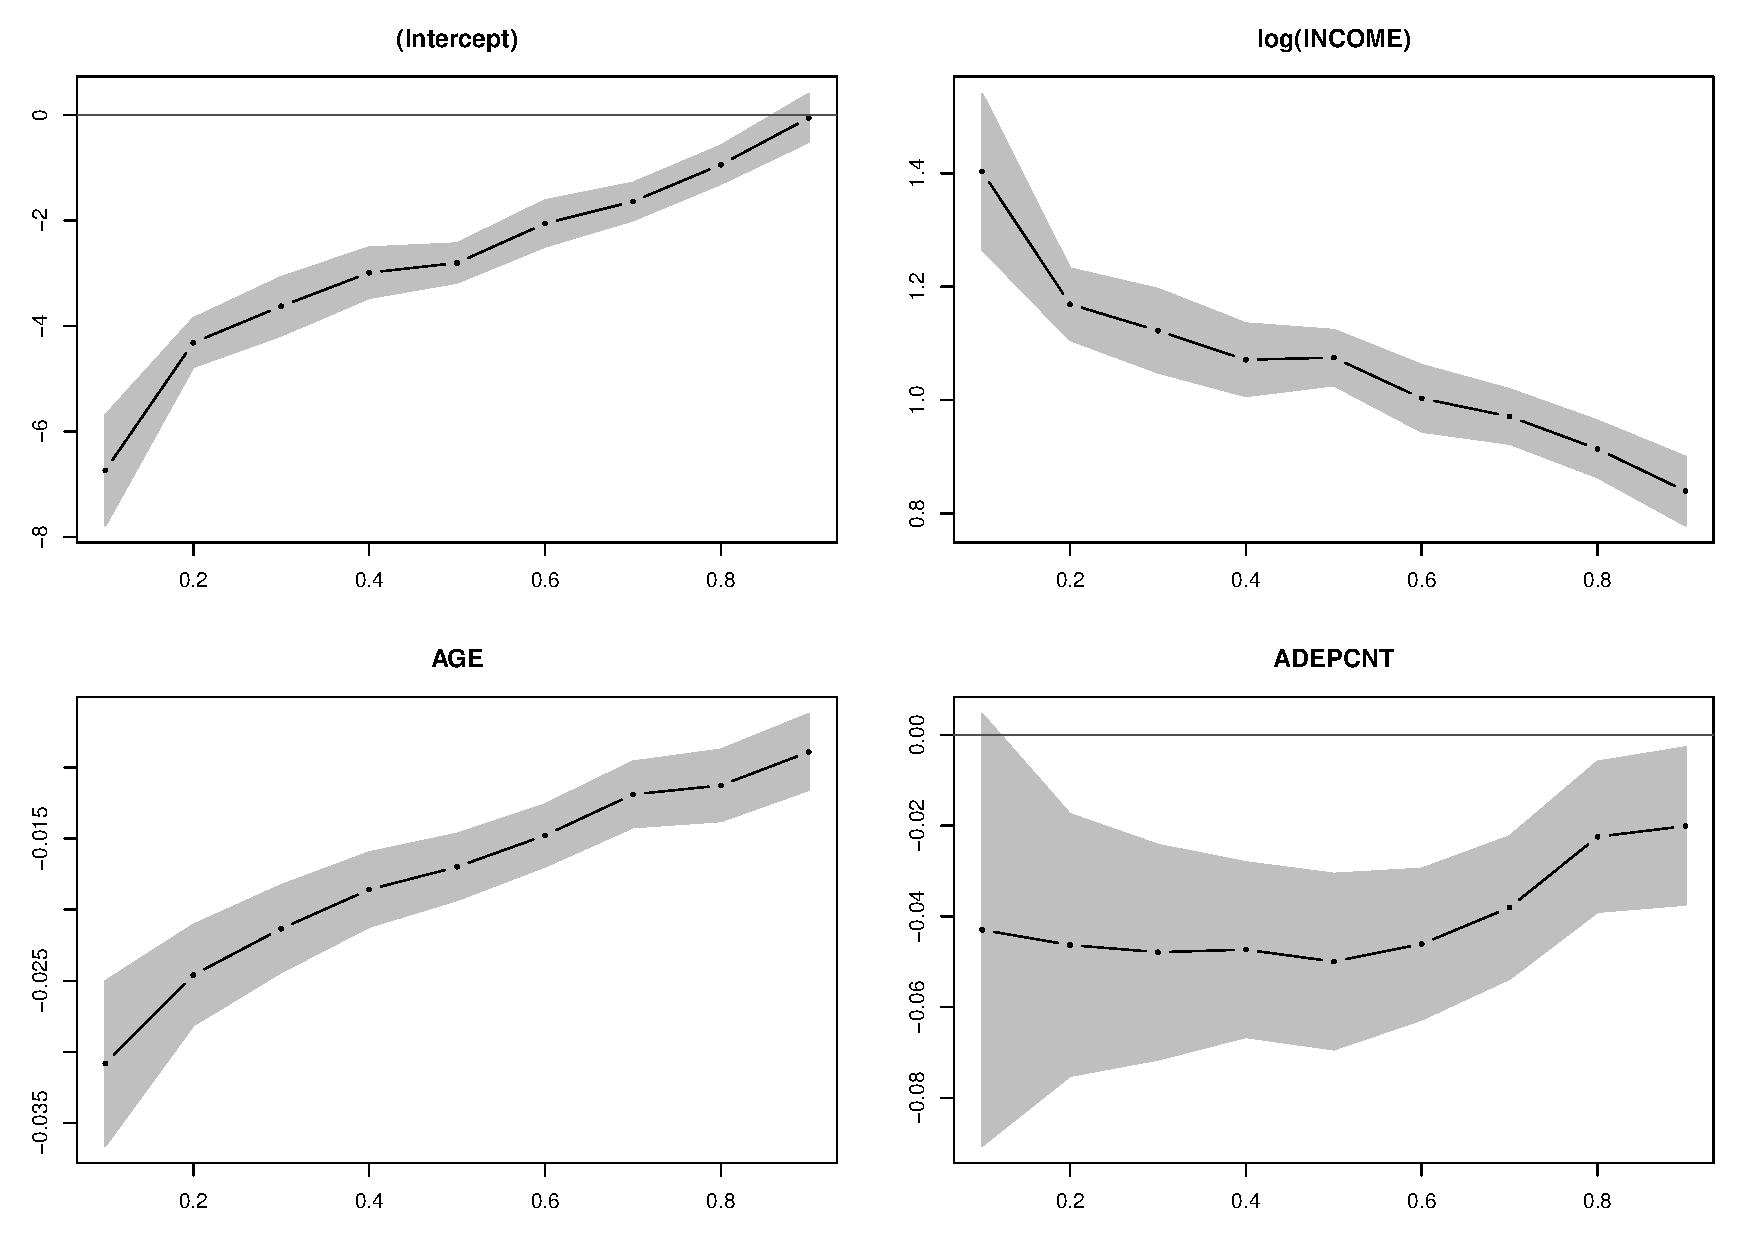
\includegraphics[width=10cm, height=6.7cm]{img/quantil_regression.pdf}
\end{frame}
%---------------------------------
\section{Predictions from a regression model}
\begin{frame}{Predictions from a model}
    \bigskip
    \begin{itemize}
        \item Predictions from a CLRM (repetition from BSc courses)
        \bigskip
        \item Predictions: general features, $k$FCV, Variance vs. Bias
    \end{itemize}
\end{frame}
%---------------------------------------------
\subsection{Predictions from a CLRM (repetition from BSc courses)}
\begin{frame}{Predictions - basics}
\begin{itemize}
\item CLRM and its estimate:
\begin{align}\nonumber
y & = \beta_1 + \beta_2 x_2 +\beta_3 x_3 + \dots + \beta_K x_K + u\\ \nonumber
\hat{y} & = \hat{\beta}_1 + \hat{\beta}_2 x_2 +\hat{\beta}_3 x_3 + \dots + \hat{\beta}_K x_K \\ \nonumber
\end{align}
\item Prediction of expected value: 
\begin{align}\nonumber
\hat{y}_p & = E(y|x_1 = 1, x_2 = c_2,\dots,x_K = c_K)\\ \nonumber
\hat{y}_p & = \hat{\beta}_1 + \hat{\beta}_2 c_2 +\hat{\beta}_3 c_3 + \dots + \hat{\beta}_K c_K  \nonumber
\end{align}
\item Rough (underestimated) confidence interval for the expected value prediction: (95\%): $\hat{y}_p \pm 2 \times \textnormal{s.e.}(\hat{y}_p)$. \\ (Rule of thumb) 
\end{itemize}
\end{frame}

%---------------------------------------------

\begin{frame}{Predictions - basics}
$\textnormal{s.e.}(\hat{y}_p)$ can be obtained by reparametrization:

\vspace{0.5cm}
\begin{itemize}
\item Reparametrized CLRM:
$$y^*=\beta^*_1 + \beta^*_2 (x_2 -c_2) + \beta^*_3(x_3 - c_3) + \dots + u$$
\item The following holds:
\begin{align} \nonumber
 \hat{y}_p &= \hat{\beta_1^*} \\ \nonumber
 \textnormal{s.e.}(\hat{y}_p ) &= 
   \textnormal{s.e.}(\hat{\beta_1^*}), \quad i.e. \\ \nonumber
 \textnormal{var}(\hat{y}_p) &= \textnormal{var}(\hat{\beta}_1^*)
\end{align} 
\end{itemize}
\end{frame}

%---------------------------------------------

\begin{frame}{Predictions - basics}
\begin{itemize}
\item Predicted and actual values of $y_p$:
\begin{align}\nonumber
\hat{y}_p &  = \hat{\beta}_1 + \hat{\beta}_2 c_2 + \hat{\beta}_3 c_3 + \dots + \hat{\beta}_K c_K\\ \nonumber
y_p & = \beta_1 + \beta_2 c_2 + \beta_3 c_3 + \dots+\beta_K c_K + u_p \nonumber
\end{align} 
\item Prediction error
$$\hat{e}_p = y_p - \hat{y}_p = (\beta_1 + \beta_2 c_2 + \beta_3 c_3 + \dots+\beta_K c_K) + u_p - \hat{y}_p$$
\item Prediction error variance
$$\textnormal{var}(\hat{e}_p) = \textnormal{var}(u_p) + \textnormal{var}(\hat{y}_p)$$
because~~$\textnormal{var}(\beta_1 + \beta_2 c_2 + \beta_3 c_3 + \dots+\beta_K c_K)=0$
\end{itemize}
\end{frame}

%---------------------------------------------

\begin{frame}{Predictions - basics}
\begin{itemize}
\item In CLRM, homoscedasticity holds, $\sigma^2 = \textnormal{var}(u_p)$: \\

\begin{itemize}
\item $\textnormal{var}(\hat{e}_p) = \sigma^2 + \textnormal{var}(\hat{y}_p)$
\vspace{0.2cm}
\item We estimate $\sigma^2$ from the original CLRM as $(\textit{SSR}/(n-K))$
\vspace{0.2cm}
\item We get $\textnormal{var}(\hat{y}_p)$ from the reparametrized LRM
\end{itemize}
\vspace{0.5cm}
\item Standard prediction error:
\begin{itemize}
\vspace{0.2cm}
 \item $\textnormal{s.e.}(\hat{e}_p) = \sqrt[]{\textnormal{var}(\hat{e}_p)}$
\end{itemize}
\vspace{0.5cm}
\item Prediction interval (95\%)
\vspace{0.2cm}
\begin{itemize}
\item $\hat{y}_p \pm t_{0.025} \times \textnormal{s.e.}(\hat{e}_p) $
\end{itemize}
\end{itemize}
\end{frame}

%---------------------------------------------

\begin{frame}{Predictions - basics}
\begin{itemize}
\item Prediction with logarithmic dependent variable
\begin{align}\nonumber
\log(y) &= \beta_1 + \beta_2 x_2 + \dots + \beta_K x_K + u\\\nonumber
\widehat{\log(y)} &= \hat{\beta}_1 + \hat{\beta}_2 x_2 + \dots + \hat{\beta}_K x_K 
\end{align}
$\hat{y} =e^{\widehat{\log(y)}}$ systematically underestimates $\hat{y}$ , \\
\vspace{0.3cm}
we can use a correction: $\hat{y}=\widehat{\alpha}_0 e^{\widehat{\log(y)}}$ \\
\vspace{0.3cm}
where $\widehat{\alpha}_0 = n^{-1} \sum_{i=1}^n \exp(\hat{u}_i)$ \\
\vspace{0.3cm}
is a consistent (not unbiased) estimator of $\exp{(u)}$.
\end{itemize}
\end{frame}

%---------------------------------------------
\begin{frame}{Predictions - basics (Matrix form)}
Prediction based on estimated model:\\
\vspace{0.3cm}
$\hat{y}_p = \bm{x}_{p}^\prime \hat{\bm{\beta}}$\\
\vspace{0.3cm}
Difference between prediction and actual $y_p$ value:\\
\vspace{0.3cm}
$\hat{e}_p \,=\, \hat{y}_p - y_p
  \,=\, \bm{x}_{p}^\prime \hat{\bm{\beta}} - \bm{x}_{p}^\prime \bm{\beta} - u_p
  \,=\, \bm{x}_{p}^\prime (\hat{\bm{\beta}} - \bm{\beta}) - u_p$\\
\vspace{0.3cm}
If $\hat{\bm{\beta}}$ is unbiased estimator for $\bm{\beta}$, \\
$\hat{y}_p$ is an unbiased estimator for $y_p$ value:\\
\vspace{0.3cm}
$E(\hat{e}_p) \,=\, E(\hat{y}_p - y_p)
   \,=\, \bm{x}_{p}^\prime E(\hat{\bm{\beta}} - \bm{\beta}) + E(-u_p) =0$\\
\vspace{0.3cm}
and the variance of $\hat{e}_p$ can be expressed as:\\
\vspace{0.3cm}
$E(\hat{e}_p^2) \,=\,\textnormal{var}(\hat{e}_p)
   \,=\, \bm{x}_{p}^\prime \textnormal{var}(\hat{\bm{\beta}})\bm{x}_{p} + \textnormal{var}(u_p) $
\end{frame}

%---------------------------------------------

\begin{frame}{Predictions - basics (Matrix form)}
Variance of $\hat{e}_p$ (continued):
\begin{equation*}
\begin{aligned}
\textnormal{var}(\hat{e}_p) \,&=\,
  \bm{x}_{p}^\prime \textnormal{var}(\hat{\bm{\beta}})\bm{x}_{p} + \textnormal{var}(u_p)\\
 \,&=\,
   \bm{x}_{p}^\prime \left[ \sigma^2 \left( \bm{X}^\prime \! \bm{X}  \right)^{-1} \right] \bm{x}_{p} + \textnormal{var}(u_p)\\
   & \textnormal{substitute $\sigma^2, \textnormal{var}(u_p)$ with $\hat{\sigma}^2$ (homoscedasticity)}\\
  \,&=\,
   \underbrace{\bm{x}_{p}^\prime \left[ \hat{\sigma}^2 \left( \bm{X}^\prime \! \bm{X}  \right)^{-1} \right] \bm{x}_{p}}_{\hat{\sigma}_p^2}
   + \hat{\sigma}^2
\end{aligned}
\end{equation*}
With growing sample size (asymptotically), \\
$\textnormal{var}(u_p) = \hat{\sigma}_p^2 + \hat{\sigma}^2$ converges to $\hat{\sigma}^2$\\
$\dots$ $\textnormal{plim} \, \hat{\bm{\beta}} = \bm{\beta} \,\,\,\, \leftrightarrow \,\,\,\, 
  \textnormal{plim} \, \hat{\sigma}_p^2 = 0$\\ \medskip
  (Note: recall consistency of the OLS estimator under A1--A5 conditions \& for the CLRM model - i.e. under A1--A6.)

\end{frame}

%---------------------------------------------
\begin{frame}{Predictions - basics (Matrix form)}
Variance of $\hat{e}_p$ (continued):
\begin{equation*}
\begin{aligned}
\textnormal{var}(\hat{e}_p) \,&=\,
\bm{x}_{p}^\prime \left[ \hat{\sigma}^2 \left( \bm{X}^\prime \! \bm{X}  \right)^{-1} \right] \bm{x}_{p}
   + \hat{\sigma}^2\\
   & \textnormal{after re-arranging, $\textnormal{s.e.}(\hat{e}_p)$ may be written as}\\
   &~\\
   \textnormal{s.e.}(\hat{e}_p) \,&=\, \hat{\sigma} \cdot \,  
   \sqrt[]{1+ \bm{x}_{p}^\prime \left( \bm{X}^\prime \! \bm{X}  \right)^{-1} \bm{x}_{p}~} \,,\\
   &\textnormal{which relates to the individual prediction error. }\\~&~\\
   &\textnormal{For mean prediction errors (considering $\hat{\sigma}_p^2$ only): }\\
   \textnormal{s.e.}(\widetilde{e}_p) \,&=\, \hat{\sigma} \cdot \,  
   \sqrt[]{~~~~ \bm{x}_{p}^\prime \left( \bm{X}^\prime \! \bm{X}  \right)^{-1} \bm{x}_{p}~} \,.\\
\end{aligned}
\end{equation*}

\end{frame}

%---------------------------------------------
\begin{frame}{Predictions - basics (Matrix form)}
Prediction intervals: individual vs. mean value predictions:\\
\vspace{0.3cm}
\textbf{Individual prediction:} $y_p \in \hat{y}_p \pm t^*_{\alpha/2} \times \textnormal{s.e.}(\hat{e}_p)$\\
\vspace{0.3cm}
\textbf{Mean value:} \hspace{1.7cm} $y_p \in \hat{y}_p \pm t^*_{\alpha/2} \times \textnormal{s.e.}(\widetilde{e}_p)$

\begin{figure}
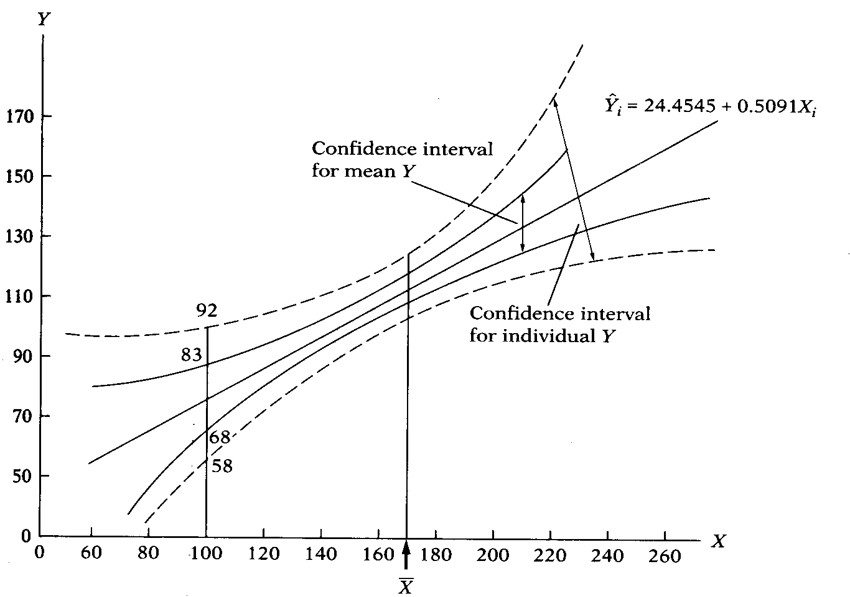
\includegraphics[width=0.6\textwidth]{img/P3_PredError.jpg}
\end{figure}

\end{frame}

%---------------------------------------------
\subsection{Predictions: general features, \textit{k}FCV, Variance vs. Bias}
\begin{frame}{Predictions -- general discussion:}
\begin{itemize}
\item Reliability of predictions: \\ \bigskip

\begin{itemize}

\item we work with estimated parameters \\(if we generalize from the CLRM paradigm, finite/small sample properties of estimators may difficult to describe),
\medskip
\item model parameters can change in time \\(discussed separately in next Block -- see Chow tests),
\medskip
\item predictions include ``individual'' random errors.
\end{itemize}
\vspace{0.3cm}
\item Impacts of random errors on predictions of individual values are usually much bigger than the impacts of variance in estimated parameters.
\end{itemize}
\end{frame}
%---------------------------------------------

\begin{frame}{Mean Squared Error of prediction}

We can generalize the previous discussion on predictions by considering both biased and unbiased predictors and by allowing for different functional forms and complexity levels in predictive models. \\ \bigskip 
Predictions may be compared/evaluated using:

\medskip
\begin{itemize}
   \item $\textit{MSE} = E
   \left[ \left( y_i - \hat{f}(\bm{x}_i) \right)^2 \right]$\\
   \smallskip
   where $\hat{f}(\bm{x}_i)$ is the prediction that $\hat{f}$ generates for the $i$-th regressor set. Here, $\hat{f}$ represents a general class of predictors (linear, non-linear, non-parametric, etc.) and it may produce either biased or unbiased predictions
\end{itemize}
\end{frame}
%---------------------------------------------
\begin{frame}{Variance vs. Bias trade-off}
Population equation example: $~y = \textnormal{sin}(x)+u$
\vspace{-1cm}
\begin{figure}
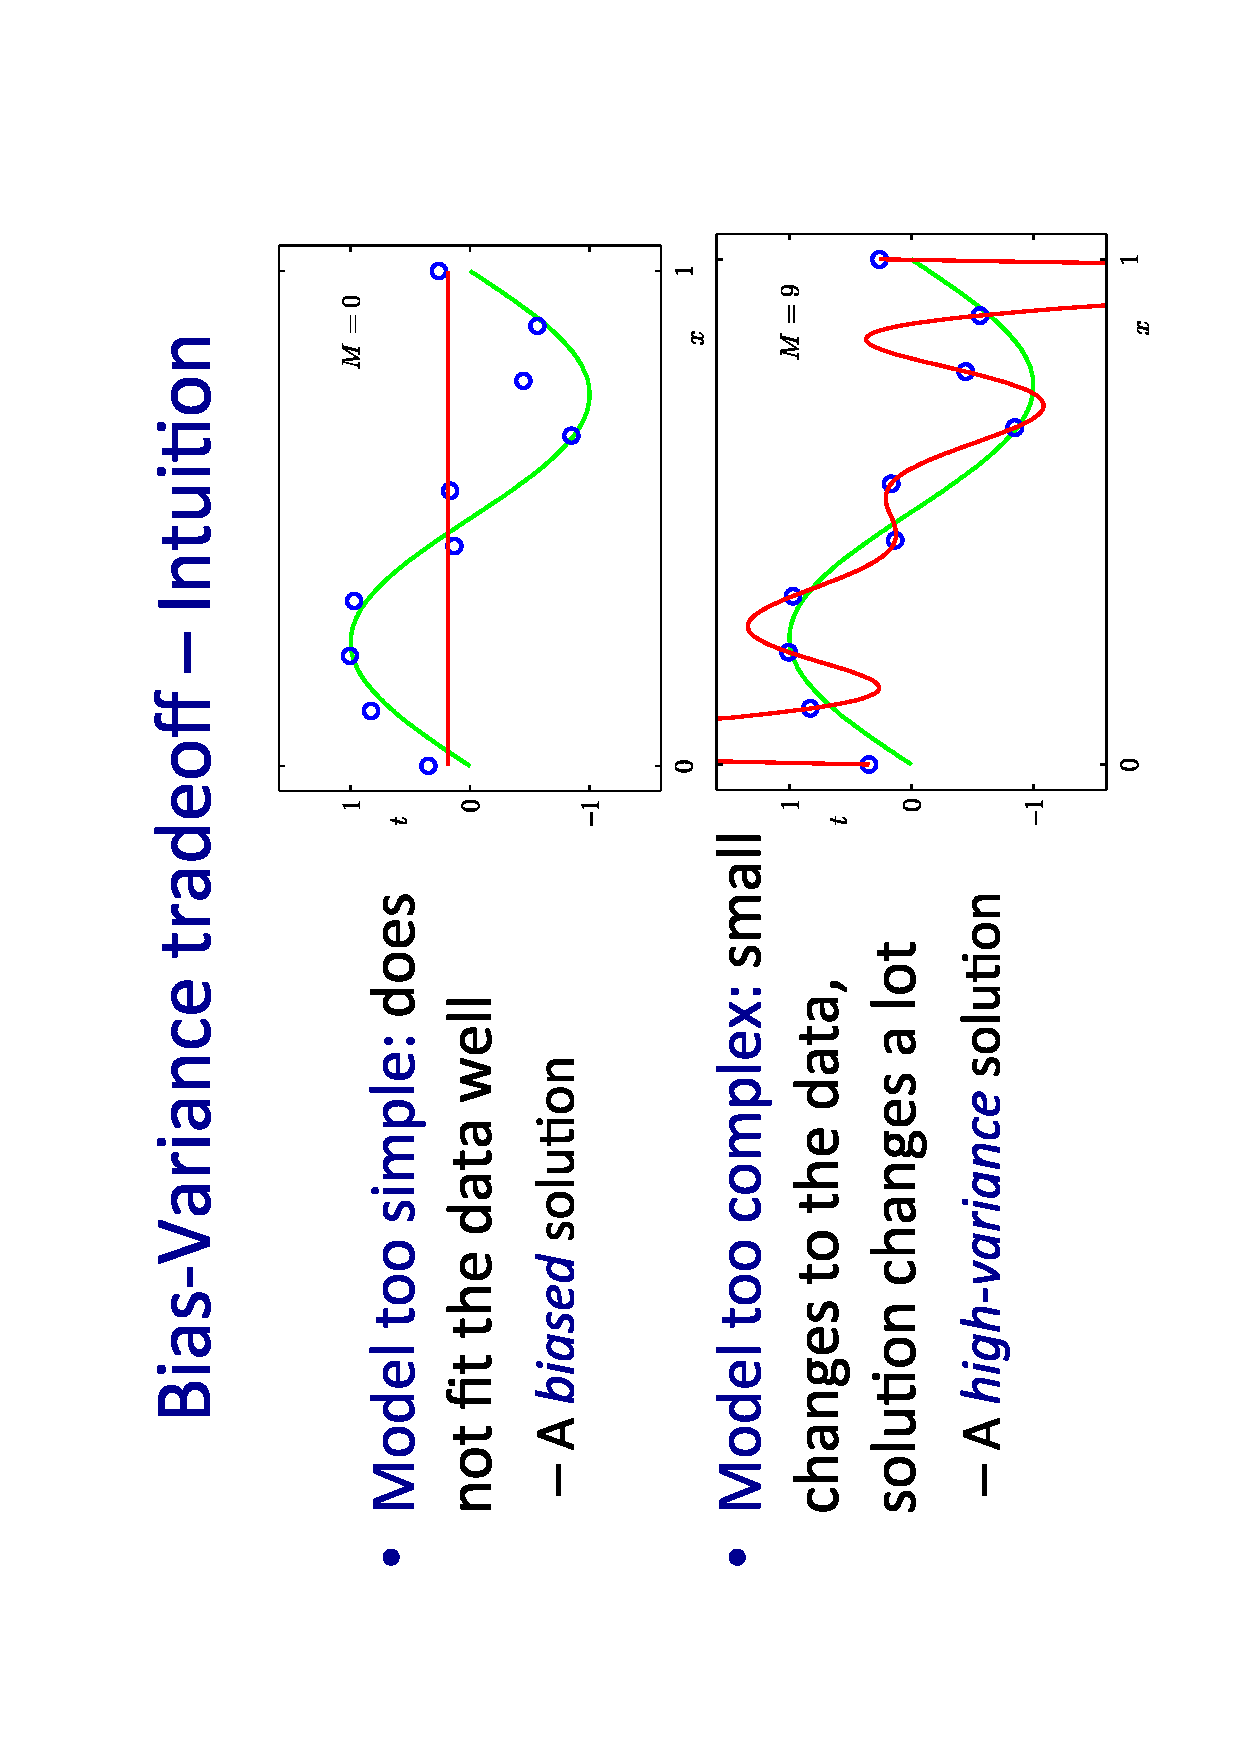
\includegraphics[angle=270,trim = 0cm 1cm 0cm 0cm, clip,width=0.9\textwidth]{img/VarBias.pdf}
\end{figure}
\end{frame}
%---------------------------------------------
\begin{frame}{Train sample \& Test sample}

Suppose we fit a model $\hat{f}(\bm{x})$ to some training data $\textnormal{Tr}=\left\lbrace y_i, \bm{x}_i \right\rbrace _1 ^n$ and we wish to see how well it performs.

\begin{itemize}
\item We could compute $\textit{MSE}$ over $\textnormal{Tr}$:
$$ \textit{MSE}_{\textnormal{Tr}} = \frac{1}{n}
   \sum_{i \in \textnormal{Tr}}
   \left[y_i - \hat{f}(\bm{x}_i) \right]^2 $$
\end{itemize}

When searching for the ``best'' model by minimizing $ \textit{MSE}$, the above statistic would lead to over-fit models.
\medskip
\begin{itemize}
\item Instead, we should (if possible) compute the $ \textit{MSE}$ using fresh test
data $\textnormal{Te}=\left\lbrace y_i, \bm{x}_i \right\rbrace _1 ^m$:
$$ \textit{MSE}_{\textnormal{Te}} = \frac{1}{m}
    \sum_{i \in \textnormal{Te}}
   \left[y_i - \hat{f}(\bm{x}_i) \right]^2 $$
\end{itemize}
\end{frame}
%------------------------------------------------
\begin{frame}{Variance vs. Bias trade-off}
Suppose we have a model $\hat{f}(\bm{x})$, fitted to some training data $\textnormal{Tr}$ and let $\left\lbrace y_0, \bm{x}_0 \right\rbrace$ be a test observation drawn from the population. If the true model is $y_i = f(\bm{x}_i) + \varepsilon_i$, \\ with $f(\bm{x}_i)= \textnormal{E}(y_i | \bm{x}_i )$,
then the $\textbf{expected test MSE}$ can be decomposed into:\\
\medskip
$E(\textit{MSE}_0)
   = \textnormal{var}(\hat{f}(\bm{x}_0))
   + [\textnormal{Bias\,}(\hat{f}(\bm{x}_0))]^2
   + \textnormal{var}(\varepsilon_0),$

where\\
\smallskip
$\textnormal{Bias\,}(\hat{f}(\bm{x}_0)) 
       = E[\hat{f}(\bm{x}_0)]
       - f(\bm{x}_0)$,\\
$\varepsilon_0$ is the irreducible error: $E(\textit{MSE}_0) \geq \varepsilon_0$,\\ 
all three RHS elements are non-negative,\\
\smallskip
The above equation refers to the average test \textit{MSE} that we would obtain if we repeatedly estimated $f(\bm{x})$ using a large number of training sets and then tested each $\hat{f}(\bm{x})$ at $\bm{x}_0$.
\end{frame}
%---------------------------------------------
\begin{frame}{Variance vs. Bias trade-off}
$E(\textit{MSE}_0)
   = \textnormal{var}(\hat{f}(\bm{x}_0))
   + [\textnormal{Bias\,}(\hat{f}(\bm{x}_0))]^2
   + \textnormal{var}(\varepsilon_0),$\\

\begin{figure}
\centering
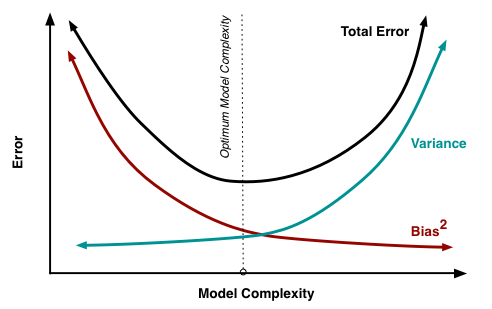
\includegraphics[trim = 0cm 0cm 0cm 0cm, clip,width=0.6\textwidth]{img/biasvariance.png}
\end{figure}

\small{This is an illustration, $\textnormal{var}(\varepsilon_0)$ not shown explicitly. \\(lies at the /asymptotic/ minima of Variance and $\textnormal{Bias}^2$)}
\end{frame}
%------------------------------------------------
\begin{frame}{$k$-Fold Cross Validation}
\begin{itemize}
\item Training error ($\textit{MSE}_{\textnormal{Tr}}$) can be calculated easily. 
\item However, $\textit{MSE}_{\textnormal{Tr}}$ is not a good approximation for the $\textit{MSE}_{\textnormal{Te}}$ (out-of sample predictive properties of the model).
\item Usually, $\textit{MSE}_{\textnormal{Tr}}$ dramatically underestimates $\textit{MSE}_{\textnormal{Te}}$.
\end{itemize}
\bigskip
Cross-validation is based on re-sampling (similar to bootstrap).\\
\medskip
Repeatedly fit a model of interest to samples formed from the training set \& make ``test sample'' predictions, in order to obtain additional information about predictive properties of the model.\\
\end{frame}
%---------------------------------------------
\begin{frame}
\frametitle{$k$-Fold Cross Validation}

\begin{itemize}
  \item In $k$-Fold Cross-Validation ($k$FCV), the original sample is randomly partitioned into $k$ roughly equal subsamples (divisibility). 
  \smallskip
  \item One of the $k$ subsamples is retained as the test sample, and the remaining $(k-1)$ subsamples are used as training data. 
  \smallskip
  \item The cross-validation process is then repeated $k$ times \\(the $k$ folds), with each of the $k$ subsamples used exactly once as the test sample. 
  \smallskip
  \item The $k$ results from the folds can then be averaged to produce a single estimation. 
  \smallskip
  \item $k = 5$ or $k=10$ is commonly used.
\end{itemize}  
\end{frame}
%------------------------------------------------
\begin{frame}{$k$-Fold Cross Validation}
\begin{center}
$k$FCV example for CS data \& $k=5$: \\
(random sampling, no replacement)
\begin{figure}
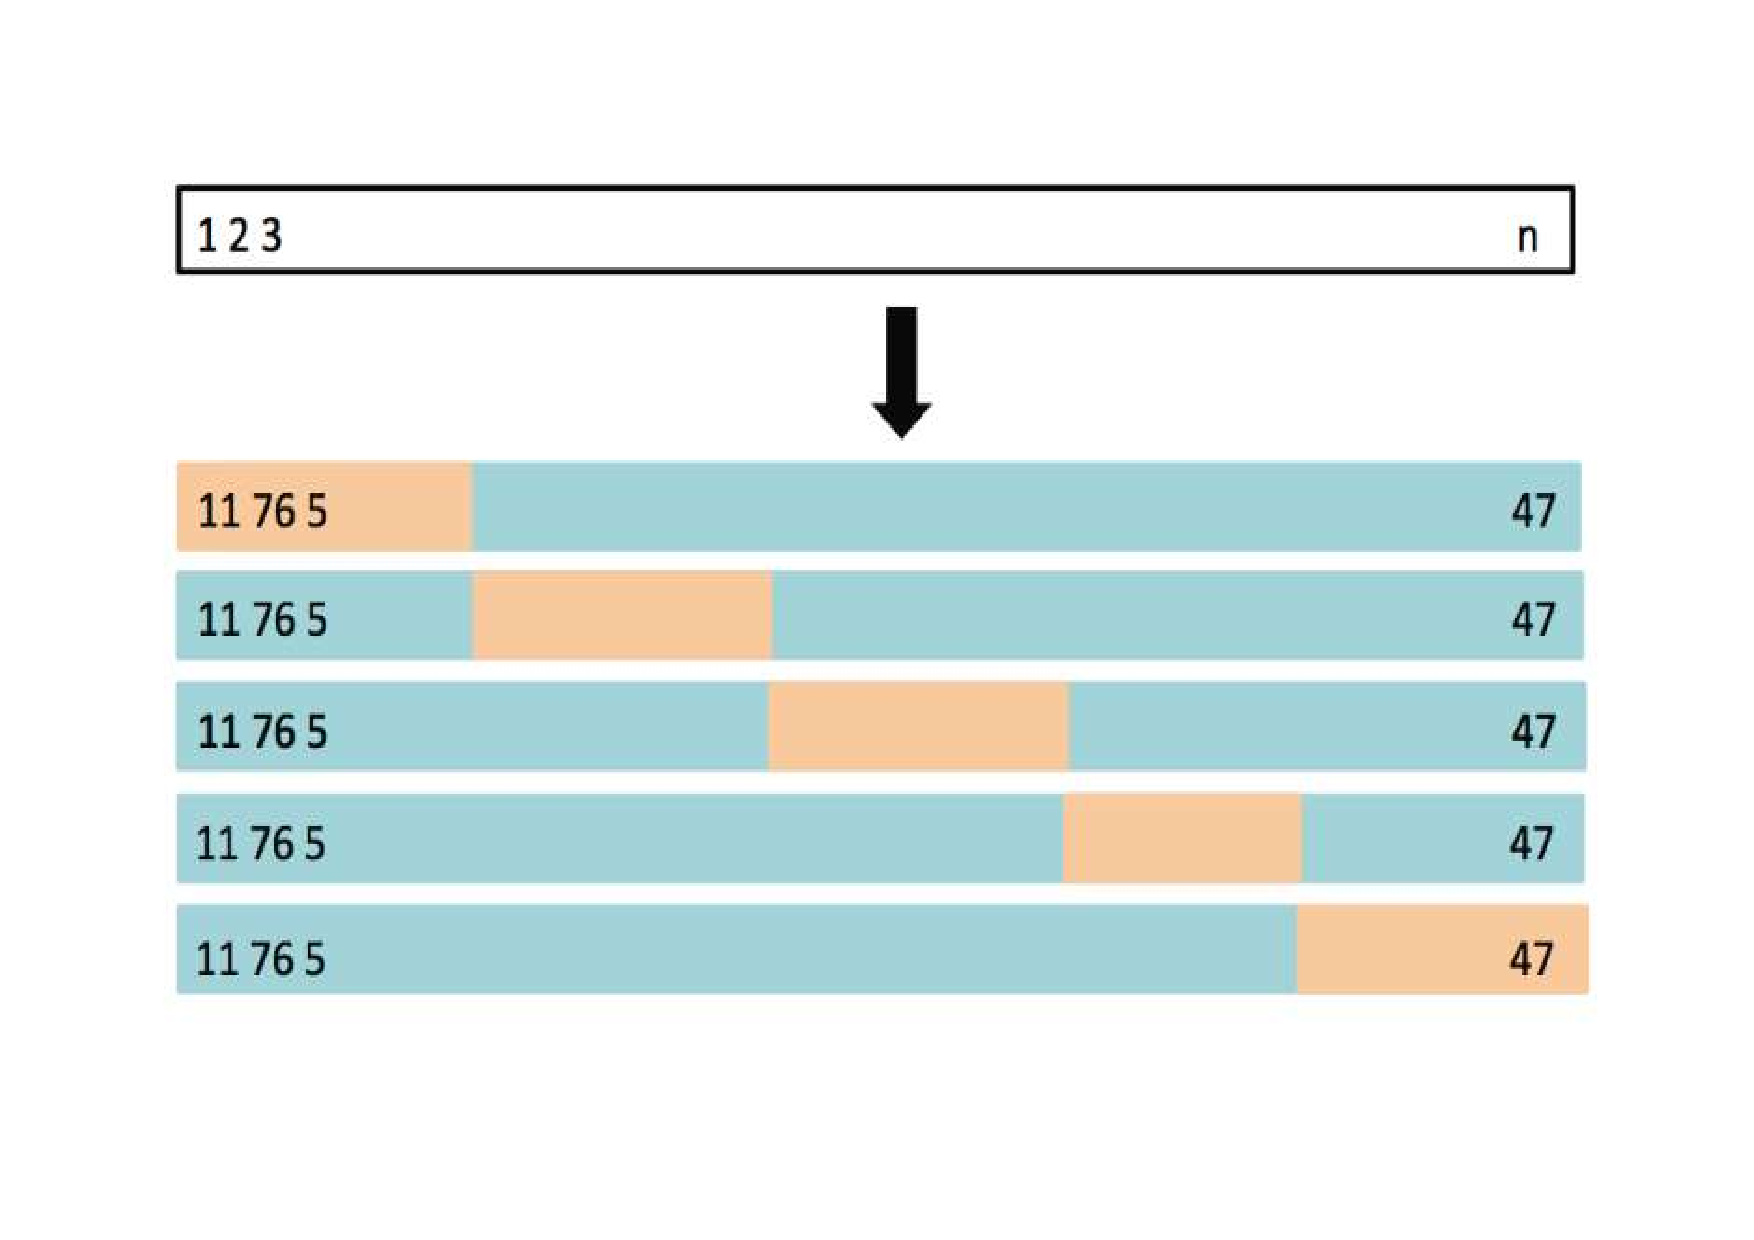
\includegraphics[width=0.7\textwidth]{img/kFCV2.pdf}
\end{figure}
In TS, a similar ``Walk forward'' test procedure may be applied.
\end{center}
\end{frame}
%------------------------------------------------
\begin{frame}{$k$-Fold Cross Validation}
$ \textit{CV}_{(k)}= \frac{1}{k}\displaystyle\sum_{s=1}^{k} \textit{MSE}_s ,$
\vspace{0.3cm}
\begin{itemize}
\item [where] $\textit{CV}_{(k)}$ is the cross-validated estimate of \textit{MSE},
\item[ ] $k$ is the number of folds used (e.g. 5 or 10),
\item[ ] $\textit{MSE}_s = \frac{1}{m_s} \sum_{i \in C_s}^{}(y_i - \widehat{y}_i)^2 $ 
\item[ ] $m_s$ is the number of observations in the $s$-th test sample
\item[ ] $C_s$ refers to the $s$-th set of test sample  observations. 
\end{itemize}
\vspace{0.3cm}
As we evaluate predictions from two or more models, 
\\we look for the lowest $\textit{CV}_{(k)}$. 
\end{frame}
\end{document}